\glsreset{co2hb}
\chapter{\texorpdfstring{\gls{co2hb}}{Carbamino-Haemoglobin (CO2Hb)} Optical Properties}\label{chap:co2hb}

\begin{tldrbox}
	
	\gls{co2} blood transport follows three different pathways: as a dissolved gas, as bicarbonate ions, or as \gls{co2hb} (and other carbamate compounds). An equilibrium exists between these three quantities and blood pH. Thus, determining blood \gls{co2hb} concentration would give valuable insights for total blood \gls{co2} content estimation. The non-invasive determination of the concentration of certain haemoglobin species can already be achieved by pulse oximetry, which leverages the oxidation dependence of haemoglobin's absorption spectrum to estimate the relative fractions of \gls{hb} and \gls{o2hb}. Thus, it was expected that a similar technique, termed pulse \emph{carbametry}, could be envisioned for transcutaneous \gls{co2hb} concentration measurement, given that \gls{hb} and \gls{co2hb} absorption spectra would be different.
	
	Alas, \gls{co2hb} spectrophotometry revealed no exploitable difference between the latter spectra, even if those results still have the merit of being the first report of \gls{co2hb} absorption spectrum. Additional research was conducted to assess the feasibility of transcutaneous haemoglobin fluorescence measurements but also yielded negative results. Consequently, this research avenue was abandoned, and further chapters focus on transcutaneous gaseous \gls{co2} diffusion and sensing.
	
	\tcblower
	
	\hyperref[chap:intro]{Previous chapter} \hfill \hyperref[chapter:toc]{Main Table Of Content (TOC)} \hfill \hyperref[chap:tcco2]{Next chapter}
	
\end{tldrbox}

\vspace{.3cm}\hrule\vspace{.1cm}\hrule\vspace{.3cm}

\textbf{Ce qu'on s'était dit:} intro sur Propriétés optiques de la carbamino-hémoglobine et // avec oxy Hb, Carbamétrie pulsée, Fluorescence de l’Hb, Conclusion

\textbf{Ce que j'ai fait:} intro sur le transport du CO2 (et de l'O2 de façon plus anecdotique), permet d'introduire la spectro de l'hémoglobine en général et l'oxymétrie de pouls, puis co2hb, mesures / carbamétrie pulsée, tentatives de mesures en fluo puis conclusion.

\vspace{.3cm}\hrule\vspace{.1cm}\hrule\vspace{.3cm}

\section{Blood Gases Transport in the Body}\label{sect:co2hb:blood_gases}

Before delving into the intricacies of \gls{co2hb} optical properties, some basic knowledge of gaseous transport throughout the body is necessary, and is the object of the present section. As mentioned in the previous chapter, cellular respiration consumes \gls{o2}---which needs to be brought from the outer air to the cells that need it---and produces \gls{co2}---which in turns need to be drained away from the cells that produces it so as to be exhaled in the outer air. These gaseous exchanges are predominantly performed by the lungs\footnote{The skin is also involved in human respiration, accounting for about 1--3\% of total exchanges in adults\cite{fitzgerald1957}, and up to 6--9\% in newborns\cite{evans1986}, cutaneous \gls{co2} diffusion will be discussed in great details in Chapter~\ref{chap:tcco2}.}, which act as a large exchange membrane between the diaphragm-ventilated air, and the capillary blood that perfuses them.

In a nutshell, \gls{o2}-rich and \gls{co2}-poor arterial blood is first pumped by the heart throughout the body, where it goes from arteries to arterioles and finally capillaries to perfuses all organs. There, \gls{o2} is released from the red blood cells---\aka{} erythrocytes---of the capillary blood to the surrounding cells that will consume it and release \gls{co2} as a result. This \gls{co2} is then carried away by the exiting capillary blood, which is subsequently collected by venules and drained by veins, carrying the \gls{o2}-depleted, \gls{co2}-rich venous blood back to the heart. The latter then pumps it through the lungs, wherein it will replenish in \gls{o2} from---and release some of its \gls{co2} into---the alveolar air. This \gls{o2}-rich and \gls{co2}-poor blood then enters the heart again, to be pumped throughout the whole body, and the cycle goes on. This is, of course, a somewhat simplified view of what actually happens, and I can only recommend the curious reader to dig into Michael Levitzky's \textit{Pulmonary Physiology}\cite{levitzky2003pulmonary}, or Andrew Lumb's  \textit{Nunn's Applied Respiratory Physiology}\cite{nunns} for a much more complete overview of the subtleties of the respiratory function in humans.

This crude outline of respiratory physiology emphasises the crucial role of blood for gas transport, as the latter must be able to convey large quantities of \gls{o2} and \gls{co2} between the lungs and the perfused organs. This is achieved by various mechanisms, which are presented in Figure~\ref{fig:co2hb:blood_gases_transport} with their relative contributions to gas transport, and described in the following sections.

% This is already said in introduction, although left here in case anyone (most likely myself when re-reading this) whants additionnal references.
%Please note that all the upcoming considerations always refer to arterial blood and \textbf{not} to venous blood (unless specified otherwise). Indeed, even if arterial and venous blood gases contents are correlated\cite{brandenburg1998}, they strongly differ in the general case, and fluctuations of the venous blood can occur due to physical exercise for instance\cite{casaburi1989}\footnote{For more information about the arteriovenous gap, see Section~\hl{XX}}. Thus, the information of clinical interest is that of arterial blood.

\begin{figure}
	\centering
	\includegraphics{1_main_matter/co2hb_figures/tikz/out/blood_gases_transport.pdf}
	\caption{Blood gases transport for \gls{o2} and \gls{co2}.}
	\label{fig:co2hb:blood_gases_transport}
\end{figure}

\subsection{\texorpdfstring{\gls{o2}}{O2} Transport}\label{subsect:co2hb:o2_transport}

\gls{o2} is present in human blood in two different forms: as dissolved gas (only 3\% of the total amount of \gls{o2} in blood) and combined with haemoglobin (the remaining 97\%). Although \gls{o2} is not at the heart of this thesis, the following developments are relevant to introduce the notions of solubility, dissociation curves, and haemoglobin (oxygen) binding. This short digression on \gls{o2} transport is also mandatory to understand the pulse oximetry principle---presented in Section~\ref{sect:co2hb:pulse_oximetry}---that is extrapolated to \gls{co2} with the concept of pulse carbametry---introduced in Section~\ref{sect:co2hb:pulse_carbametry}.

\subsubsection{As dissolved gas}

\gls{o2} is present in blood as a dissolved gas according to Henry's law---named after the English chemist William Henry (1774-1836)---which states that the amount of dissolved gas in a liquid is proportional to its partial pressure in the gas phase\cite{henry1803}. The coefficient linking the partial pressure of the gas phase to the amount of gas dissolved in the liquid is known as the \emph{solubility}. The latter is function of the nature of the considered gas and liquid, as well as the temperature. For instance, \gls{o2} solubility in human blood at 37{\degree}C is known to be equal to 0.023~mL of \gls{o2} per mL of blood for 1~atm (760 mmHg)\footnote{Although I tried to stick with SI units throughout this thesis, pressures are conventionally expressed in mmHg in medical practice. The reader should bear in mind that 1~atm = 1.01325~bar = 101~325~Pa = 760~mmHg. Also volumes of gases are noted with the gas name in subscript, \eg{} mL$_{\ce{O2}}$ or mL$_{\ce{CO2}}$.} of \gls{po2}\cite{resp_care}. Given a normal \gls{pao2} of 100~mmHg\cite{malatesha2007}, the concentration of \gls{o2} dissolved in human arterial blood is\footnote{The symbol \enquote{M} stands for 1~molar, \ie{} 1~mol.L$^{-1}$.}:
\begin{equation}
	\ce{[O2_{(gas)}]} = 3 \text{ mL}_{\ce{O2}}.\text{L}^{-1} = 1.2 \text{ mM}
\end{equation}

As pointed out by Lewitzky\cite[p.~143]{levitzky2003pulmonary}, if dissolved \gls{o2} were the only oxygen source in blood, the required cardiac output to match the body consumption in \gls{o2} should be around 83~L.min$^{-1}$. Knowing that the maximum cardiac output is about 25~L.min$^{-1}$, dissolved oxygen is clearly not sufficient for the needs of human metabolism.

\subsubsection{Combined with haemoglobin}

Indeed, dissolved oxygen is only the top of the iceberg, and most blood-carried \gls{o2} is in fact bound to haemoglobin in the erythrocytes. Haemoglobin is an iron-containing metalloporphyrin that is composed of four subunits called hemes. The latter act as fixation sites for \gls{o2}, each heme being able to bind to one \gls{o2} molecule\cite{antonini1970}. Haemoglobin concentration in healthy human blood is about 14~g.dL$^{-1}$, and given that 1~g of haemoglobin can carry up to 1.39~mL$_{\ce{O2}}$, human blood can theoretically carry up to about 200~mL$_{\ce{O2}}$.L$^{-1}$\cite[Chap.~11]{nunns} (\ie{} $\approx80$~mM). Compared to the 3~mL$_{\ce{O2}}$.L$^{-1}$ of dissolved \gls{o2}, this explains the 98\%--2\% repartition for \gls{o2} transport in blood presented in Figure~\ref{fig:co2hb:blood_gases_transport}. Since the overwhelming majority of blood \gls{o2} is transported bound to haemoglobin, only the latter mechanism is considered in the next paragraph.

\subsubsection{The oxygen-haemoglobin dissociation curve}

The binding of haemoglobin with \gls{o2} can be described by the oxygen-haemoglobin dissociation curve, represented in Figure~\ref{fig:co2hb:barcroft_curve}. First evidenced by Joseph Barcroft in 1909\cite{barcroft1909}---hence its alternate designation as the \enquote{Barcroft curve}---it represents the percentage of \gls{o2}-carrying haemoglobin---\ie{} \gls{o2hb}---over the total \emph{active} haemoglobin concentration---\ie{} \gls{o2hb} and \gls{hb}. This quantity---referred to as the oxygen saturation---is defined as follows:
\begin{equation}\label{eq:co2hb:sat_def}
	\text{oxygen saturation} = \frac{[\text{\gls{o2hb}}]}{[\text{\gls{o2hb}}] + [\text{\gls{hb}}]}
\end{equation}

When measured in arterial blood, the latter quantity becomes the \gls{o2sat}. Of note, there has been some confusion in the definition of the oxygen saturation in the past decades, with the denominator in Equation \ref{eq:co2hb:sat_def} being replaced by the \emph{total} haemoglobin concentration instead of the \emph{active} one. Although those two quantities are close enough in the absence of dishaemoglobins---such as \gls{methb} or \gls{cohb}---the gap between them widens as their concentration in blood increases\cite{toffaletti2007}---\eg{} in case of methaemoglobinemia\cite{souza2008} or \gls{co} poisoning\cite{hampson2018}, for instance.

\begin{figure}
	\centering
	\includegraphics{1_main_matter/co2hb_figures/tikz/out/barcroft_curve.pdf}
	\caption[The oxygen-haemoglobin dissociation curve.]{The standard oxygen-haemoglobin dissociation curve, as given by Severinghaus at \pH~=~7.40 and T~=~37{\degree}C\cite{severinghaus1966}. For reference, the arterial \gls{po2} is about 100~mmHg while the venous one is about 40~mmHg. However, the corresponding points were not indicated on the curve since \textit{(i)} \pH{} is slightly lower in venous than in arterial blood, and \textit{(ii)} the oxygen dissociation curve is \pH-sensitive, shifting to the right as \pH{} decreases\cite[Chap.~7]{levitzky2003pulmonary}.}
	\label{fig:co2hb:barcroft_curve}
\end{figure}

Yet, granted that the total haemoglobin concentration is known and there is neither significant dishaemoglobins concentrations nor arterial \pH{} changes, the oxygen-haemoglobin dissociation curve can be used to directly convert between a given \gls{o2sat} and the corresponding \gls{pao2} and \gls{o2} concentration\cite[Chap.~11]{nunns}. This explains why measuring \gls{o2sat} non-invasively has gathered significant efforts for decades, leading to the advent of pulse oximetry---as we shall see in Section~\ref{sect:co2hb:pulse_oximetry}.

\subsection{\texorpdfstring{\gls{co2}}{CO2} Transport}\label{subsect:co2hb:co2_transport}

Blood conveys \gls{co2} under three different forms: \textit{(i)} as a dissolved gas, \textit{(ii)} bound to proteins---mainly haemoglobin---in the form of carbamate compounds, and \textit{(iii)} as bicarbonate ions---\ie{} \ce{HCO3-}. This section briefly details the three corresponding mechanisms before discussing the equilibra that take place between them, explaining why the determination of blood \gls{co2hb} concentration may be relevant to \gls{paco2} estimation.

% Carbon dioxide transport : https://doi.org/10.1093/bjaceaccp/mki050 a short introductory text on the topic

\subsubsection{As dissolved gas}

Similarly to \gls{o2}, \gls{co2} can also dissolve in blood according to Henry's law, the solubility coefficient of \gls{co2} in plasma at 37{\degree}C being 0.231~mM.kPa$^{-1}$ (0.0308~mM.mmHg$^{-1}$)\cite[Table~10.1]{nunns}. A normal \gls{paco2} in arterial blood\footnote{It seems to be common practice to use the solubility of \gls{co2} in plasma for both the erythrocytes and the whole arterial blood\cite{geers2000}. I could not find appropriate justifications for this in the literature, although the root cause may be that \textit{(i)} erythrocyte are mainly bags of haemoglobin-rich salty water, and that \textit{(ii)} \gls{co2} plasma solubility is also close to that of water, so that \textit{(iii)} what really matters for \gls{co2} solubility is only the presence of water.} of 5.3~kPa (40~mmHg) thus leads to a dissolved \gls{co2} concentration

\begin{equation}
	\ce{[CO2_{(gas)}]}=1.2\text{~mM} (= 3.1\text{~mL$_{\ce{CO2}}$.L$^{-1}$})
\end{equation}

\hl{J'ai vraiment galéré à trouver autre chose que la solubilité dans le plasma (et toutes les sources secondaires que j'ai trouvées qui parlent de sang, citent une source primaire qui parle de plasma), je veux bien vos lumières là dessus / si jamais vous avez une bonne justification de ça je suis preneur.}

\subsubsection{Combined with haemoglobin}\label{subsect:co2hb:co2_transport:carbamates}

\gls{co2} can also combine chemically with the terminal amine groups of blood proteins---\ie{} plasma proteins and haemoglobin---according to the following scheme:

\begin{equation}
	\schemestart
	\chemname{\chemfig{R-N(-[1]H)=[7]O}}{Terminal\\amine group}
	\+
	\chemname{\ce{CO2}}{Carbon\\dioxide}
	\quad\xrightleftharpoons{}\quad
	\chemname{\chemfig{R-N(-[7]CO{O^-})-[1]H}}{Carbamino\\compound}
	\+
	\chemname{\ce{H+}}{Proton}
	\schemestop
\end{equation}

When \gls{co2} binds to haemoglobin, the so-obtained molecule is called \glsreset{co2hb}\gls{co2hb}, while for other proteins the more general terms \emph{carbamate compound} or \emph{carbamino carriage} are generally used. For reference, plasma total protein levels are normally in the 6--8~g.dL$^{-1}$ range\cite{vanslyke1950, ditzel1971}---which would translate into whole blood concentration of 13--18~g.dL$^{-1}$ assuming a 45\% haematocrit---while normal haemoglobin concentration in blood is about 13.2$\pm$1.1\female{} / 14.7$\pm$1.4\male{}~g.dL$^{-1}$ (mean value $\pm$ \gls{sd})\cite{us_hematological2005}. Nevertheless, despite plasma proteins and haemoglobin concentrations being relatively close, the latter accounts for over twice as much \gls{co2} transport as the former, owing to the greater haemoglobin capacity for binding to \gls{co2} molecules. Indeed, under a 5.3~kPa (40~mmHg) \gls{paco2}, \gls{co2hb} accounts for a concentration of \gls{co2} in arterial blood of 0.75~mM, while the carbamate compounds of plasma proteins account only for 0.30~mM\cite{geers2000}. Overall, the carbamate-bound \gls{co2} content of whole arterial blood is thus about 1.05~mM (or 2.7~mL$_{\ce{CO_2}}$.dL$^{-1}$).

Of note, certain textbooks---\eg{} \textit{Nunn's [\dots]}\cite[Chap.~10]{nunns}---completely neglect plasma protein carbamates, presenting only \gls{co2hb} when mentioning carbamino carriage. Given the orders of magnitude involved, this may be acceptable in first approximation for educational reasons, and also explains why only \gls{co2hb} was mentioned in Figure~\ref{fig:co2hb:blood_gases_transport}. For further information about \gls{co2hb} formation mechanisms, the curious reader may refer to the works of Van Kampen\cite{vankampen1972_phd}, Gros \etal{}\cite{gros1981}, and Blake \etal{}\cite{blake2022}.

Regarding modelling the formation mechanism of carbamino compounds, while the following formula appears to be valid for plasma proteins carbamates\cite{klocke1987}
\begin{equation}
	\ce{[R-NHCOO^-]} = \sum_{i=\alpha, \varepsilon} \frac{n_i \cdot [\text{proteins}] \cdot \ce{[CO2_{(gas)}]}}{\ce{[CO2_{(gas)}]} + \frac{\ce{[H+]}}{K_{c_i}} + \frac{\ce{[H+]}^2}{K_{c_i} \cdot K_{z_i}} }
\end{equation}
no equivalent formulae exists for haemoglobin binding. Indeed, although attempts have been made to obtain a similar formula for \gls{co2hb} concentration, these were not successful because most of them ignored the crucial role of \gls{23dpg}---\aka{} 2,3-DPG---in haemoglobin \gls{co2} binding\cite{gros1981, klocke1987}. To the best of my knowledge, a single exception resides in the work of Perrella,  who suggests a rational function of \ce{[CO2_{(gas)}]} and [\gls{23dpg}] in his short 1975 letter\cite{perrella1975a}, although \emph{(i)} the latter holds only for a \pH{} of 7.4---which is slightly above that of inner erythrocytes (7.2, as mentioned above)---and \emph{(ii)} Perrella might have just fitted an equation with enough degrees of freedom to his data, which could result into a poor generalisation of his approach.

\subsubsection{As bicarbonate ions}\label{subsect:co2hb:bicarb}

The total \gls{co2} concentration in arterial blood being around 21.50~mM (or 55~mL$_{\ce{CO_2}}$.dL$^{-1}$), the dissolved \gls{co2} (1.2~mM) and carbamate-bound \gls{co2} (1.05~mmol.L$^{-1}$) only account for roughly $10\%$ of the overall amount of \gls{co2}\cite{geers2000}. The $90\%$ left are indeed present in the form of bicarbonate ions which are created through the hydration and dissociation of \gls{co2}, which is a di-acid:

\begin{equation}\label{eq:co2hb:carb_disso}
	\ce{CO2 + H2O <=>T[carbonic][anhydrase] H2CO3 <=> H+ + HCO3- ( <=> 2H+ + CO3^2- )}
\end{equation}

Of note, the second dissociation of \gls{co2} into carbonate ions (\ce{CO2^2-}) has a \pKa{} above 9\footnote{The latter is 10.25 in water at 25{\degree}C, but decreases markedly with increasing temperature and ionic strength\cite{hastings1925, macinnes1933}.}, and carbonate ions are thus present in negligible concentration in human blood, hence the parentheses around the corresponding reaction. The creation of carbonic acid (\ce{H2CO3}) from dissolved \gls{co2} is normally very slow in water, however the presence of carbonic anhydrase---an enzyme vastly present inside the erythrocytes---speeds up the reaction by a factor of $13\,000$ up to $25\,000$\cite{levitzky2003pulmonary}\cite{geers2000}. Thus, carbonic acid accounts for a negligible part of \gls{co2} in blood (only 0.0017~mmol.L$^{-1}$\cite[Table~10.2]{nunns}) and the equilibrium actually takes place between dissolved \gls{co2} and bicarbonate ions. In other words Equation~\ref{eq:co2hb:carb_disso} is virtually equivalent to:
\begin{equation}\label{eq:co2hb:carb_disso_eq}
	\ce{CO2 + H2O <=> H+ + HCO3-}
\end{equation}
in human blood. This equilibrium is described by the following Henderson-Hasselbach equation
\begin{equation}\label{hh_eq_co2}
	\pH = \pKa + \log_{10} \left( \frac{\ce{[HCO_3^-]}}{\ce{[CO2_{(gas)}]}} \right) = \pKa + \log_{10} \left( \frac{\ce{[HCO_3^-]}}{s \cdot \mathrm{P}_{\ce{CO_2}}} \right)
\end{equation}
wherein $\pKa=6.10$ in human body at 37{\degree}C\cite{messier1975, geers2000}, $s \approx 30$~{\textmu}M.mmHg$^{-1}$ is the solubility coefficient of \gls{co2} in plasma\cite[Table~10.1]{nunns} and P$_{CO_2}$ its partial pressure. A normal \pH{} value for human blood is considered to be between 7.35 and 7.45\cite{rossana}. Taking a \pH{} value of 7.4 and a \gls{paco2} of 5.3~kPa (40~mmHg) thus leads to a bicarbonate concentration \ce{[HCO3^-]} of about 24~mM in plasma. Given that the erythrocytes have an intracellular \pH{} of 7.2\cite{kummerow2000, jensen2004}, this leads to a lower erythrocytic \ce{[HCO3^-]} of about 15~mM. Taking into account the relative proportions of plasma and erythrocytes in blood---\ie{} the haematocrit---the total bicarbonate concentration in arterial blood is about 19~mM. There again, this latter value---when compared with the respective concentrations of dissolved \gls{co2} and carbamate-bound \gls{co2}---explains the 90\%-5\%-5\% repartition for \gls{co2} transport in blood presented in Figure~\ref{fig:co2hb:blood_gases_transport}.

\subsubsection{\texorpdfstring{\gls{co2}}{CO2} repartition and equilibria}

To wrap it all up, \gls{co2} is present in the body under three distinct forms\footnote{Indicative values for arterial blood are given as undersets (or oversets when needed), all numerical values come from above cited references, except for [\gls{23dpg}] which comes from Meen \etal{}\cite{meen1981}. The \enquote{extra} and \enquote{intra} terms refer to extra-cellular---\ie{} plasmatic---and intra-cellular---\ie{} erythrocytic---values, respectively.}:
\begin{enumerate}
	\item Dissolved as a gas, according to Henry's law:\begin{equation}
		\underset{\text{1.2~mM}}{\ce{[CO2_{(gas)}]}} = \underset{\text{0.231~mM.kPa$^{-1}$}}{\alpha} \cdot \underset{\text{5.3~kPa (40~mmHg)}}{\text{\gls{paco2}}}
	\end{equation}
	\item Bound to proteins, forming carbamate compounds with both plasma proteins (\ce{R-NHCOO-}) and haemoglobin (\gls{co2hb}). No mathematical model describes whole blood haemoglobin carriage in the literature, although the following kind of relation can reasonably be assumed:
	\begin{equation}\label{eq:co2hb:unknown_carb}
		\underset{\text{1.05~mM}}{[\text{Carb}]} = f\Bigl(
		\underset{
			\begin{subarray}{l}
				\text{7.4 extra}\\
				\text{7.2 intra}
			\end{subarray}}{\pH},
		\underset{\text{6--8~g.dL$^{-1}$}}{[\text{proteins}]}, 
		\underset{\text{13--15~g.dL$^{-1}$}}{[\text{Hb}]}, 
		\underset{\text{4--5~mM}}{[\text{\gls{23dpg}}]_{\text{intra}}},
		\underset{\text{1.2~mM}}{\ce{[CO2_{(gas)}]}} \Bigr)
	\end{equation} wherein $f$ is a rational function and [Carb] denotes the \gls{co2} concentration bound to carbamates (\ie{} $[\text{Carb}] = [\ce{R-NHCOO-}] + [\text{\gls{co2hb}}]$).
	\item As bicarbonate ions (\ce{HCO3-}) accounting for the vast majority of blood \gls{co2} transport:\begin{equation}
		\underset{\begin{subarray}{l}
				\text{24~mM extra}\\
				\text{15~mM intra}
			\end{subarray}}{\ce{[HCO3^-]}} = \underset{\text{1.2~mM}}{\ce{[CO2_{(gas)}]}}\cdot 10^{\overset{\begin{subarray}{l}
					\text{7.4 extra}\\
					\text{7.2 intra}
			\end{subarray}}{\pH} - \overset{6.1\vphantom{p}}{\pKa}}
	\end{equation}
\end{enumerate}

Alas, the task of deriving a global equilibria for whole blood \gls{co2} content from these three equations is by no mean a trivial one. Indeed, variations in \gls{paco2} usually entail \pH{} changes both in the plasma and the erythrocytes which are not necessarily of the same order of magnitude. Thus, in practice, many more equilibria take place between \gls{paco2}, \pH, \ce{[HCO3^-]}, [proteins], and [Hb] than the few above-described ones, not to mention other species such as \gls{23dpg}, plasma phosphates, and extra- and intra-erythrocytic ions---\ie{} \ce{Na+}, \ce{Mg^2+}, \etc{}. Navigating through this chemical \mhiddenlink{https://ia802907.us.archive.org/27/items/bosch-garden/Bosch\%20garden.jpg}{hell} has generated significant research efforts for decades, resulting into the creation of several whole blood acido-basic models, with major contributions from Siggaard-Andersen\cite{siggaard1974acid} and Stewart\cite{stewart1981understand} in the seventies and early eighties. Recent improvements were added within the last two decades, and provided faithful modelling of blood acid-base equilibria, taking into account \gls{paco2} and \gls{o2sat} (cross-)influences\cite{rees2010, oneill2017, jezek2018}. Yet, the resulting models are not easily usable by common mortals due to the large number of equations and parameters they involve, and they often gain in accuracy what they loose in readability.

Consequently, I will limit myself here to presenting the simple cases of respiratory acidosis and alkalosis along with their influences on the total \gls{co2} content of whole arterial blood, but the reader is now warned that this is a gross simplification of a much more complex and nuanced picture. To do so, the following two equations from the well-known Davenport diagram were used\cite[Fig.~17]{davenport1974abc}:
\begin{equation}
	\begin{array}{ll}
		\ce{[HCO3^-]} = \alpha \cdot \text{\gls{paco2}}\cdot 10^{\pH - \pKa} & \alpha = \text{0.231~mM.kPa$^{-1}$}\\
		\ce{[HCO3^-]} = m - s \cdot (\pH - 7.40) & m = \text{24~mM}\\
		& s = \text{31.6~mM(.\pH$^{-1}$)}
	\end{array}
\end{equation}
Then, the following hypotheses were made:
\begin{itemize}
	\item[$\mathcal{H}_1$:] \pH{} changes occurs with the same magnitude in plasma and erythrocytes, \ie{} if plasma \pH{} decreases from 7.4 to 7.3, erythrocytic \pH{} also goes down from 7.2 to 7.1.
	\item[$\mathcal{H}_2$:] the proportion of intra- / extra-erythrocytic \ce{[HCO3^-]} remains constant, \ie{} 27\% / 73\% (using Geers's data\cite{geers2000}).
\end{itemize}
Doing so made it feasible to derive single \ce{[HCO3^-]} and \pH{} values for any given \gls{paco2}. Then, using Mochizuki's data for total \gls{co2} blood content\cite{mochizuki1982}\footnote{First equation, using B=0.45. This equation was chosen because it yielded results in-between those of Tazawa \etal{}\cite{tazawa1983} and those of Loeppky \etal{}\cite{loeppky1983}, short of a better heuristic.}, Figure~\ref{fig:co2hb:co2_dissociation_curve} could be plotted considering fully oxygenated arterial blood with a plasmatic \pH{} of 7.4 at equilibrium. The latter figure represents the so-called \gls{co2} dissociation curve---by analogy with the oxygen-haemoglobin dissociation curve---along with carbamate and dissolved \gls{co2} contributions to the total blood \gls{co2} content.

\begin{figure}
	\centering
	\includegraphics{1_main_matter/co2hb_figures/tikz/out/co2_disso_curve.pdf}
	\caption[\gls{co2} dissociation curve.]{Stack plot of the respective contributions of dissolved \gls{co2}, carbamate compounds, and bicarbonate ions to the total arterial whole-blood \gls{co2} content. The upper curve in black is the so-called \gls{co2} dissociation curve, with the normal arterial blood equilibrium marked with a black dot. Again, this curve was obtained using strong hypotheses and is given here for information only.}
	\label{fig:co2hb:co2_dissociation_curve}
\end{figure}

This figure illustrates what happens in case of respiratory acidosis, for instance: a decrease in ventilation entails an increase in \gls{paco2}, which translates into higher concentrations of carbamates, bicarbonate ions, and dissolved \gls{co2}, while the opposite happens in case of respiratory alkalosis. Of particular interest (point (2.) of the box below), Figure~\ref{fig:co2hb:co2_dissociation_curve} depicts the positive effect of \gls{paco2} on blood carbamates content---and thus on [\gls{co2hb}]---already reported in the literature\cite{bauer1972, perrella1975a, gros1976}.
\begin{keypointbox}
	The idea at the very heart of the present chapter was thus the following:
	\begin{enumerate}
		\item if we can find a non-invasive mean to measure [\gls{co2hb}] and
		\item if we can uncover a satisfactory relation between [\gls{co2hb}] and \gls{paco2},
		\item then we should be able to perform non-invasive \gls{paco2} measurements.
	\end{enumerate}
	To this end, I began my research with (1.): finding a non-invasive measurement technique for [\gls{co2hb}]. By analogy, this led me to investigate the basic principles of pulse oximetry.
\end{keypointbox}

\subsection{Disclaimer on the Above Considerations}\label{sect:co2hb:abg_disclaimer}

As mentioned above, the afore developments are of course a gross simplification of the equilibria involved in blood gas transport, and many well-known mechanisms have not been detailed here. In particular the \gls{o2} and \gls{co2} binding properties of the haemoglobin molecule are function of its oxygenation and carbamation states, as well as of the surrounding pH and \gls{23dpg} concentrations. This translates in practice into the notorious Bohr---first described in 1904 by the Danish physiologist Christian Bohr (1881-1911)\cite{bohr1904}---and Haldane---named after the Scottish physiologist John Scott Haldane (1860-1936) who described it in 1914\cite{haldane1914}---effects. The curious reader may refer to Chapter 10 and 11 of \textit{Nunn's ...}\cite{nunns} for a more wide-angled, educational view of the situation, or may read the excellent reviews by Geers \etal{} on \gls{co2}\cite{geers2000} and by Mairbaürl \etal{} on \gls{o2}\cite{mairbaurl2012}, for more technical and profound insights.

\mfrin{}Of note, some of the above-discussed aspects are still in need for further clarification. In particular, a better model for the formation-dissociation of carbamate compounds would be welcome, and is still an open research avenue\cite{blake2022}. Thorough modelling of the whole blood acid-base equilibrium including respiratory and metabolic influences is also still an open research field, and the creation of an open-source, easily implementable---\ie{} by mean of a fully sourced (in terms of literature references used to derive its parameters) \gls{api} implemented using a popular programming language such as Python---appears to be highly desirable. In this direction, the recent works of O'Neill and Ježek appears quite promising\cite{oneill2017, jezek2018}, although they chose closed (Matlab) or confidential (Modelica) programming languages, and only Ježek provided what is closer to a script than to a proper \gls{api}.

\section[Hb. Optical Prop. and Their App. to Pulse Oximetry]{Haemoglobin Optical Properties and Their Application to Pulse Oximetry}

\subsection{Spectrophotometry of Human Haemoglobin Derivatives}\label{sect:co2hb:hb_optical_prop}

One noticeable property of the haemoglobin molecule is its strong optical absorption in the visible spectrum, which gives \myblood{} its characteristic red taint. Even better, the haemoglobin absorption spectrum depends on its oxygenation state---\ie{} \gls{hb} and \gls{o2hb} absorption spectra differ markedly---and other haemoglobin species such as \gls{cohb}, \gls{methb} or \gls{sulfhb} also have their specific spectral features, see Figure~\ref{fig:co2hb:hb_spectra}.

\begin{figure}
	\centering
	\includegraphics{1_main_matter/co2hb_figures/tikz/out/hb_spectra.pdf}
	\caption[Absorption spectra of haemoglobin derivatives from the literature.]{Haemoblobin absorption spectra. Data compiled from various sources: \gls{o2hb} and \gls{hb} spectra come from Prahl\cite{prahl1998}, while \gls{methb}, \gls{cohb}, and \gls{sulfhb} spectra come from Zijlstra \etal{}\cite{zijlstra2000}.\\\textbf{Note:} Zijlstra's coefficients were converted to molar extinction coefficients according to Prahl's recommendations. Indeed, they were initially reported as \emph{equivalents}---\aka{} \emph{quarter millimolar absorptivities}---\ie{} using haem concentration instead of haemoglobin concentration. The reader eager to indulge in haemoglobin spectrophotometry should be aware of the factor of four existing between the two quantities, one haemoglobin molecule being composed of four haems.}
	\label{fig:co2hb:hb_spectra}
\end{figure}

Spectrophotometry of human haemoglobin derivatives began as far back as the 17th century, with the pioneering works of Fracassiti\cite{fracassati1667} and Mayow\cite{mayow1674}, who both observed a change in the colour of blood depending on its exposure to ambient air\footnote{See Engelhart for an interesting early history of haemoglobin studies\cite{engelhart1827}. Further historical considerations can be found in the introduction of Assendelft's monograph\cite[Chap.~1]{assendelft1970}.}. However, it took no less than three centuries to translate these early qualitative observations into accurate quantitative measurements. In particular, we must salute the many contributions from van Assendelft, van Kampen and Zijlstra, from the University of Groningen, Netherlands. They worked relentlessly on haemoglobin spectrophotometry from the early fifties to the late nineties with two major monographs on the topic\cite{assendelft1970, zijlstra2000}. In particular, their 2000 book \textit{Visible and Near Infrared Spectra of Human and Animal Haemoglobin} condenses fifty years of research on the topic, and is an essential reading for anyone interested in haemoglobin spectrophotometry. Additional references are also given in Table~\ref{tab:co2hb:hb_biblio} with indications of covered spectral ranges and measured haemoglobin species.

\begin{table}[ht]
	\small
	\def\arraystretch{1.1}
	%\resizebox{\textwidth}{!}{
	\begin{adjustbox}{center}
		\rowcolors{3}{white}{gray!20}
		\begin{tabular}{lllrrcccccccl}
			\multirow{2}{*}{Year} & \multirow{2}{*}{Author} & \multirow{2}{*}{Ref.} & \multicolumn{2}{l}{\begin{tabular}[c]{@{}l@{}}Measurement\\ window (nm)\end{tabular}} & \multirow{2}{*}{\gls{o2hb}} & \multirow{2}{*}{\gls{hb}} & \multirow{2}{*}{\gls{cohb}} & \multirow{2}{*}{\gls{methb}} & \multirow{2}{*}{CNMetHb} & \multirow{2}{*}{\gls{sulfhb}} & \multirow{2}{*}{\gls{co2hb}} & \multirow{2}{*}{Notes} \\
			&  &  & $\lambda_{\min}$ & $\lambda_{\max}$ &  &  &  &  &  &  &  &  \Bstrut\\ \hline
			1919 & Newcomer & \cite{newcomer1919} & 241 & 700 & \checkmark & & \checkmark & \checkmark & & & & \\
			1938 & Sidwell & \cite{sidwell1938} & 230 & 780 & \checkmark & \checkmark &  &  &  &  &  & \\
			1943 & Horecker & \cite{horecker1943} & 600 & 1000 & \checkmark & \checkmark &  & \checkmark & \checkmark &  &  &  \\
			1962 & Barlow & \cite{barlow1962} & 600 & 1900 & \checkmark & \checkmark &  &  &  &  &  & \\
			1970 & Assendelft & \cite{assendelft1970} & 390 & 1000 & \checkmark & \checkmark & \checkmark & \checkmark & \checkmark & \checkmark &  & (a) \\
			1971 & Sugita & \cite{sugita1971} & 200 & 660 & \checkmark & \checkmark & & \checkmark & & & & \\
			1977 & Dijkhuizen & \cite{dijkhuizen1977} & 450 & 700 & & & & \checkmark & & \checkmark & & \\
			1978 & Waterman & \cite{waterman1978} & 370 & 650 & \checkmark & \checkmark & \checkmark & \checkmark & \checkmark &  &  & \\
			1979 & Mook & \cite{mook1979} & 600 & 1000 & \checkmark & \checkmark &  &  &  &  &  & \\
			1983 & Van Kampen & \cite{vankampen1983} & 380 & 1000 & \checkmark & \checkmark & \checkmark & \checkmark & \checkmark & \checkmark &  & (a)\\
			1988 & Wray & \cite{wray1988} & 650 & 1050 & \checkmark & \checkmark &  &  &  &  &  & \\
			1989 & Mendelson & \cite{mendelson1989} & 600 & 1000 & \checkmark & \checkmark &  &  &  &  &  & (b) \\ % b foetal
			1991 & Cope & \cite{cope1991} & 650 & 1050 & \checkmark & \checkmark &  &  &  &  &  & \\
			1991 & Zijlstra & \cite{zijlstra1991} & 450 & 1000 & \checkmark & \checkmark & \checkmark & \checkmark &  &  &  & (b) \\
			1994 & Kuenstner & \cite{kuenstner1994} & 620 & 2500 & \checkmark & \checkmark & \checkmark & \checkmark &  &  &  & \\
			1997 & Grosenbaugh & \cite{grosenbaugh1997} & 600 & 1000 & \checkmark & \checkmark &  &  &  &  &  & \\
			1997 & Kuenstner & \cite{kuenstner1994} & 2500 & 11800 & \checkmark & \checkmark & \checkmark & \checkmark &  &  &  & \\
			1998 & Prahl & \cite{prahl1998} & 250 & 1000 & \checkmark & \checkmark &  &  &  &  &  & (c)\\
			2000 & Zijlstra & \cite{zijlstra2000} & 450 & 1000 & \checkmark & \checkmark & \checkmark & \checkmark & \checkmark & \checkmark &  & (a),(b)\\
			2006 & Friebel & \cite{friebel2006} & 250 & 1100 &  & \checkmark &  &  &  &  &  & (d)\\
			2012 & Kolyva & \cite{kolyva2012} & 650 & 1000 & \checkmark & \checkmark &  &  &  &  &  & \\
			2020 & Dervieux & \cite{dervieux2020} & 235 & 1000 & \checkmark & \checkmark &  &  &  &  & \checkmark & 
		\end{tabular}
	\end{adjustbox}
	\caption[Selected works on the spectrophotometry of human haemoglobin derivatives.]{Selected works on the spectrophotometry of human haemoglobin derivatives. (a): additional dyshaemoglobins species reported$^\dagger$, (b): foetal haemoglobin also reported, (c): compiled from various data sources, (d): measurement performed on unlysed erythrocytes.\\
	$\dagger$: \gls{methb} is sometimes called haemiglobin and noted Hi, while CNMetHb refers to cyan-methaemoglobin, also called haemiglobincyanide and noted HiCN. Many more haemoglobin species exist combining the sulf-, meth- and cyan- prefixes, as detailed by Zijlstra\cite[p.~11 and Figure~2.2]{zijlstra2000}.}\label{tab:co2hb:hb_biblio}
\end{table}

Haemoglobin spectrophotometry drew the attention of many a researcher for two main reasons. First, because it allows the total haemoglobin concentration to be determined from a blood sample using the photometric cyanmethaemoglobin method\cite{vankampen1983}, which is particularly interesting from a medical viewpoint---\eg{} when focusing on anaemia\cite{neufeld2019}. Second, because the differences in absorption spectra between \gls{o2hb} and \gls{hb} can be used to non-invasively estimate a patient's \gls{o2sat}: this is the goal of pulse oximetry.

\subsection{Pulse Oximetry}\label{sect:co2hb:pulse_oximetry}

Photometric oximetry---\ie{} optically measuring the oxygen saturation of a blood sample---emerged in the early 20th century, following the afore-mentioned discovery that \gls{o2hb} and \gls{hb} had different absorption spectra. From then, it took over half a century before Aoyagi's major breakthrough, with the invention of pulse oximetry in 1974\cite{miyasaka2021}. For a thorough history of the development of both classical oximetry and pulse oximetry, I kindly redirect the curious reader to the excellent historical reviews written by Severinghaus \etal{}\cite{severinghaus1986_6, severinghaus1987_vii}\footnote{Make sure to read both papers---and not just the first one---as the second primarily serves as an erratum to the first. As a side note, those two papers are part of an heptalogy on the topic of blood gas analysis by one of the leading expert on the subject, and are worth reading from a historical viewpoint.}. For more recent developments, current medical practice, and challenges, I would rather orient them towards several publications by Jubran\cite{jubran2015}, Nitzan \etal\cite{nitzan2014}, and Tamura\cite{tamura2019}. In the remainder of this section, I will briefly outline the core principles of pulse oximetry from a more technical point of view. Further reading on the topic include Urpalainen's work, which---despite being only a master's thesis---is extremely clear and educational, making her work quite valuable for a newcomer to the field\cite[Chap.~2]{katja2011}.

To understand the basic idea behind pulse oximetry, let us consider Figure~\ref{fig:co2hb:ppg_principle}, which illustrates the following. Light is shone onto a limb---\eg{} a finger or earlobe---by mean of a \gls{led}, with an initial incident intensity $I_0$. The light entering the skin is then partially absorbed inside the tissues before it eventually exits them with an intensity $I$, which may finally be measured with a photodiode. The absorption of light by the tissue may then be quantified by plotting the absorbance---\ie{} $A=\log_{10}(I/I_0)$---of the tissues with respect to time. When doing so, the absorbance can be decomposed into two parts: \textit{(i)} a \emph{constant} signal---termed \gls{dc} from the electrical engineering / signal processing analogy---due to the absorbance of tissues, venous blood, and the volume of arterial blood that remains constant throughout a cardiac cycle and \textit{(ii)} a \emph{pulsatile} signal---termed \gls{ac}---which corresponds to the change in arterial blood volume with each heartbeat.

\begin{figure}
	\centering
	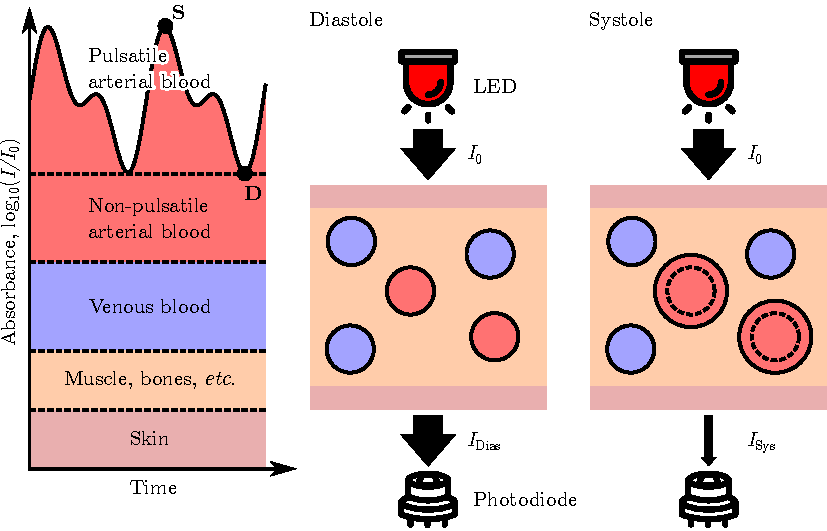
\includegraphics{1_main_matter/co2hb_figures/ppg_principle.pdf}
	\caption[Pulse oximetry principle.]{The pulse oximetry principle. \textbf{Left:} time-varying absorbance of perfused tissues, with decomposition of the said absorbance between different compartments (not to scale). Of note, the arterial blood is divided into a non-pulsatile and a pulsatile components, with the systole and diastole indicated with the \enquote{S} and \enquote{D} letters. \textbf{Center and Right:} schematised cut-views of perfused tissues during the diastole and systole. Skin, muscle, veins, and arteries are represented using the same colours as in the left-hand side diagram. Note the change in arteries diameters between the systole and the diastole, which account for the change in the amplitudes of $I_\text{Sys}$ and $I_\text{Dias}$ between the two situations.}
	\label{fig:co2hb:ppg_principle}
\end{figure}


Indeed, during diastole---the relaxed phase of the cardiac cycle---the arterial blood pressure is minimal, and the arteries thus occupies their minimum volume. At the opposite, when systole occurs---\ie{} when the heart contracts and ejects its blood content into the arteries---the arterial blood pressure is maximal, and the arterial volume increase---it is this volume variation that can be felt when taking the pulse of a person. This volume change is in fact a change in the volume of blood contained in the said arteries, and since blood is one of the most absorbing substance within human tissues\cite{jacques2013}, the latter change in blood volume in turns translate into a measurable change in tissues absorbance. This ability of measuring changes in (blood) volume by optical means is called \gls{ppg}, derived from Greek \emph{photo-} light, \emph{-plethysmo-} increasing, enlarging (relative to volume changes), and \emph{-graphy} writing.

Mathematically speaking, the absorbance of the perfused limb at a given wavelength $\lambda$ may be written
\begin{equation}
	A_\lambda(t) = - \log_{10}\left(\frac{I(t)}{I_0}\right) = A_{\lambda,\text{DC}} + \underbrace{A_{\lambda,\text{AC}}(t)}_{\mathclap{\substack{\text{pulsatile} \\ \text{arterial blood}}}}
\end{equation}
where the total absorbance $A_\lambda$ is decomposed into its \gls{dc} and \gls{ac} components. $A_{\lambda,\text{DC}}$ represents the sum of the respective absorbances of the non-varying afore-mentioned compartments---\ie{} skin, muscle and bones, venous blood, and non-pulsatile arterial blood---while $A_{\lambda,\text{AC}}$ specifically represents the absorbance of pulsatile arterial blood, \ie{}
\begin{equation}\label{eq:co2hb:beer_law}
	A_{\lambda,\text{AC}}(t) = \sum_{i} \varepsilon_{\lambda, i} \cdot \mathcal{C}_i \cdot \ell_{\lambda, i}(t)
\end{equation}
wherein $i$ represent the different absorbing species in blood (mainly haemoglobin species), $\varepsilon$ are their molar extinction coefficients, $\mathcal{C}$ their concentration, and $\ell$ the optical path taken by the illuminating light---\ie{} the length of blood that would produce the same absorbance as the sum of all the optical paths actually taken through the many arteries of the perfused limb. Note that this path length $\ell$ is time-varying, being zero during diastole, and reaching its maximal value when the systole occurs. We can study the difference between the maximum (systolic) and minimum (diastolic) absorbance value:
\begin{equation}\label{eq:co2hb:adiff_logi}
	\begin{aligned}
		A_{\lambda,\max} - A_{\lambda,\min} &= - \log_{10}\left(\frac{I_\text{Sys}}{I_0}\right) + \log_{10}\left(\frac{I_\text{Dias}}{I_0}\right)\\
		&= \log_{10}\left(\frac{I_\text{Dias}}{I_\text{Sys}}\right)
	\end{aligned}
\end{equation}
On the other hand we also have
\begin{equation}
	\begin{aligned}
		A_{\lambda,\max} - A_{\lambda,\min} &= \sum_{i} \varepsilon_{\lambda, i} \cdot \mathcal{C}_i \cdot \Delta\ell_{\lambda, i}
	\end{aligned}
\end{equation}
wherein $\Delta\ell_{\lambda, i}$ is the amplitude of $\ell_{\lambda, i}(t)$, \ie{} $\Delta\ell_{\lambda, i} = \ell_{\lambda, i, \text{Sys}} - \ell_{\lambda, i, \text{Dias}}$. Using two different \glspl{led} of wavelengths $\lambda_1$ and $\lambda_2$, the following ratio can then be computed:
\begin{equation}\label{eq:co2hb:ratio_def}
	\begin{aligned}
		R &= \frac{A_{\lambda_1,\max} - A_{\lambda_1,\min}}{A_{\lambda_2,\max} - A_{\lambda_2,\min}} = \frac{\log_{10}\left(\frac{I_{\lambda_1,\text{Dias}}}{I_{\lambda_1,\text{Sys}}}\right)}{\log_{10}\left(\frac{I_{\lambda_2,\text{Dias}}}{I_{\lambda_2,\text{Sys}}}\right)}\\
		R &= \frac{\sum_{i} \varepsilon_{\lambda_1, i} \cdot \mathcal{C}_i \cdot \Delta\ell_{\lambda_1, i}}{\sum_{i} \varepsilon_{\lambda_2, i} \cdot \mathcal{C}_i \cdot \Delta\ell_{\lambda_2, i}}
	\end{aligned}
\end{equation}

Then, the following hypotheses are made---they will be discussed later on:
\begin{itemize}
	\item[$\mathcal{H}_1$:] $\Delta\ell_{\lambda_1, i} = \Delta\ell_{\lambda_2, i}$, \ie{} the light path inside the tissues is independent of the wavelength.
	\item[$\mathcal{H}_2$:] $i\in$ [\gls{hb}, \gls{o2hb}], \ie{} the only two light-absorbing substances in arterial blood are the oxy- and deoxygenated haemoglobin species.
	\item[$\mathcal{H}_3$:] $\mathcal{C}_\text{Hb,\sc{tot}} = \mathcal{C}_\text{\gls{hb}} + \mathcal{C}_\text{\gls{o2hb}}$, wherein $\mathcal{C}_\text{Hb,\sc{tot}}$, $\mathcal{C}_\text{\gls{hb}}$, and $\mathcal{C}_\text{\gls{o2hb}}$ are the total haemoglobin, \gls{hb}, and \gls{o2hb} arterial blood concentration, respectively, \ie{} haemoglobin is either present in the form of \gls{hb} or \gls{o2hb}, and no dishaemoglobin is present. In particular, $\mathcal{H}_3$ leads to:
	\begin{equation}
		\mathcal{C}_\text{\gls{o2hb}} = \text{\gls{o2sat}} \cdot \mathcal{C}_\text{Hb,\sc{tot}} \qquad\text{and}\qquad \mathcal{C}_\text{\gls{hb}} = (1-\text{\gls{o2sat}}) \cdot \mathcal{C}_\text{Hb,\sc{tot}}
	\end{equation}
\end{itemize}

Those three hypotheses then lead to
\begin{equation}\label{eq:co2hb:rr_defsao2}
	R= \frac{\text{\gls{o2sat}} \cdot \varepsilon_{\lambda_1,\text{\gls{o2hb}}} + (1-\text{\gls{o2sat}})\cdot \varepsilon_{\lambda_1,\text{\gls{hb}}}}{\text{\gls{o2sat}} \cdot \varepsilon_{\lambda_2,\text{\gls{o2hb}}} + (1-\text{\gls{o2sat}})\cdot \varepsilon_{\lambda_2,\text{\gls{hb}}}}
\end{equation}
from which \gls{o2sat} can be expressed as:
\begin{equation}\label{eq:co2hb:spo2_formulae}
	\boxed{
	\text{\gls{o2sat}} = \frac{\varepsilon_{\lambda_1,\text{\gls{hb}}} - R \cdot \varepsilon_{\lambda_2,\text{\gls{hb}}}}{\left(\varepsilon_{\lambda_1,\text{\gls{hb}}} - \varepsilon_{\lambda_1,\text{\gls{o2hb}}}\right) - R \cdot \left(\varepsilon_{\lambda_2,\text{\gls{hb}}} - \varepsilon_{\lambda_2,\text{\gls{o2hb}}}\right)}
	}
\end{equation}

This latter relation if fundamental in pulse oximetry, as it allows to compute the \gls{o2sat} from $R$, which can itself be calculated using the right-hand-side of Equation~\ref{eq:co2hb:ratio_def} and the measured diastolic and systolic light intensities---represented in Figure~\ref{fig:co2hb:ppg_principle}---at two different wavelengths. Of note, when the \gls{o2sat} is computed by pulsed oximetry it is termed \enquote{peripheral oxygen saturation}, and noted \gls{spo2}.

\subsubsection{Alternative calculus}

There are two alternative ways of calculating \gls{spo2} which are sometimes encountered in the literature. The first one generalises Equations~\ref{eq:co2hb:adiff_logi} and \ref{eq:co2hb:ratio_def} by using the derivative of the absorbance instead of its amplitude, \ie{} turning the latter equations into
\begin{equation}
	\begin{tabular}{ccc}
		$
		\begin{aligned}
			\frac{dA_\lambda}{dt}(t) &= \overbrace{\frac{A_{\lambda,\text{DC}}}{dt}(t)}^{=0} + \frac{A_{\lambda,\text{AC}}}{dt}(t) = \sum_{i} \varepsilon_{\lambda, i} \cdot \mathcal{C}_i \cdot \frac{d\ell_{\lambda, i}}{dt}(t)\\
			&= -\frac{d\log_{10}\left(\frac{I(t)}{I_0}\right)}{dt} = -\frac{1}{I(t)}\cdot \frac{dI}{dt}(t)
		\end{aligned}
		$ & \hspace{0.6cm} and \hspace{0.6cm} & $
		R = \frac{\cfrac{dA_{\lambda_1}}{dt}(t)}{ \cfrac{dA_{\lambda_2}}{dt}(t)}
		$
	\end{tabular}
\end{equation}

This can lead to instantaneous \gls{spo2} values, without the need to wait for the end of a complete cardiac cycle\cite{vazquezjaccaud2011}. The second alternative relies on the decomposition of light intensity into its \gls{ac} and \gls{dc} parts, \ie{} using the notations
\begin{eqnarray}
	\text{DC} = I_{\text{Sys}} & \text{AC} = I_{\text{Dias}} - I_{\text{Sys}}
\end{eqnarray}
Then, equation \ref{eq:co2hb:adiff_logi} becomes
\begin{equation}
	\begin{aligned}
		A_{\lambda,\max} - A_{\lambda,\min} &= \log_{10}\left(\frac{I_\text{Dias}}{I_\text{Sys}}\right) = \log_{10} \left( \frac{\text{DC} + \text{AC}}{\text{DC}} \right) = \log_{10} \left(1 + \frac{\text{AC}}{\text{DC}}\right)\\
		&\approx \frac{\text{AC}}{\text{DC}}
	\end{aligned}
\end{equation}
using an equivalent of $\log_{10}$ in zero, because \gls{ac} is small with respect to \gls{dc} in practice. Indeed the \gls{ac}/\gls{dc} ratio---referred to as the \gls{pi}---is about 4.5\% when measured at the finger on healthy adults\cite{tapar2018, fodor2022}, but this latter figure varies widely depending on the subject's position\cite{rathgeber1996, tapar2018} or state of health\cite{sivaprasath2019}, for instance. This simplification gave $R$ the name of \emph{ratio-of-ratios}\cite{nitzan2014} because it thus becomes the ratio of two \gls{ac}/\gls{dc} ratios at wavelengths $\lambda_1$ and $\lambda_2$, \ie{}:
\begin{equation}
	R = \frac{\text{AC}_{\lambda_1} / \text{DC}_{\lambda_1}}{\text{AC}_{\lambda_2} /\text{DC}_{\lambda_2}}
\end{equation}

\subsubsection{Hypotheses validity and the calibration curve}

Hypotheses $\mathcal{H}_1$ through $\mathcal{H}_3$, although allowing the derivation of a closed-form for \gls{spo2}---and thereby possessing significant explanatory power---are in fact wildly optimistic, ad detailed below.

Regarding $\mathcal{H}_1$: $\Delta\ell_{\lambda_1, i} = \Delta\ell_{\lambda_2, i}$, significant research efforts have been put into modelling light propagation throughout the tissues. In particular, Monte-Carlo simulations conducted by Chatterjee \etal{} in a series of publications\cite{chatterjee2017, chatterjee2018, chatterjee2019, chatterjee2020} clearly demonstrate the wavelength dependency of path lengths.

$\mathcal{H}_2$---stating that \gls{hb} and \gls{o2hb} are the only light-absorbing substance in the arterial blood---and $\mathcal{H}_3$---stating that haemoglobin is either present as \gls{hb} and \gls{o2hb}---are linked together in the sense that $\mathcal{H}_2$ requires $\mathcal{H}_3$ to be true. Alas, $\mathcal{H}_3$ is not quite true, since even non-smoking healthy adults have small percentages of haemoglobin present as \gls{cohb} and \gls{methb}---about 1--2\% of \gls{cohb} and 1\% of \gls{methb}, and the latter figures can be as high as 6--8\% of \gls{cohb} for heavy smokers, or over 40\% of \gls{methb} in case of methaemoglobinaemia\cite{nordenberg1990, ashbernal2004, remigio2022}. Worse still regarding $\mathcal{H}_2$ veracity, haemoglobin is not the only light-absorbing substances in blood, with bilirubin presenting significant absorbance below 600~nm, for instance, although the latter should not be problematic except in case of severe hyperbilirubinemia\cite{beall1989, veyckemans1990, meinke2007}.

Last, but not least, all the aforementioned considerations---and in particular Equation~\ref{eq:co2hb:beer_law}---assumes that light propagation inside the blood and tissues obeys the Beer-Lambert law of absorption, \ie{} only absorption was considered, not scattering events. In actuality, human tissues---and even blood alone, for that matter---are highly scattering media\cite{jacques2013, bosschaart2014}. This, in conjunction with the inexactitude of hypotheses $\mathcal{H}_\text{1--3}$ likely explains the observed differences between the theoretical \gls{spo2}=f($R$) curve and the empirical one. Indeed, in practice, pulse oximetry manufacturers derive an empirical \gls{spo2}=f($R$) curve based on real-life hypoxia sessions on a large number of subjects instead of using Equation~\ref{eq:co2hb:spo2_formulae}\cite[Chap.~10]{webster1997design}. Of note, taking into account light scattering allows for the derivation of accurate calibration curves, at the expense of much more complex calculations than the above-presented ones\cite{schmitt1991}, and the so-obtained curves are still influenced by total haematocrit\cite{mannheimer1997}.

\subsubsection{Wavelengths selection and the multi-wavelength approach}\label{sect:co2hb:spo2_multiwl}

A crucial step when building a pulse oximeter, which is also key to understanding the pulse carbametry-related considerations of the next section, is that of appropriate wavelength selection. Just as bygone researchers wondered about the optimal wavelength pair to use in static oximetry\cite{nilsson1960, mook1969}, the advent of pulse oximetry sparked similarly intense discussions on the very same topic\cite[Chap.~4]{damianou1995, mannheimer1997, vazquezjaccaud2011}. Usually, $\lambda_1$ and $\lambda_2$ are chosen in the red and infra-red regions of the spectrum---\eg{} 660 and 940~nm---although other combinations have been proposed relatively close to those---\eg{} 660 and 805, or 735 and 890~nm\cite{mannheimer1997, li2014}.

One of the limitation of the above-presented two-wavelengths approach is its inability to quantify haemoglobin species other than \gls{hb} and \gls{o2hb}---\eg{} \gls{cohb} and \gls{methb}. Even worse, high concentrations of the latter dyshaemoglobins could distort \gls{spo2} measurements\cite{wukitsch1987, ralston1991}. To mitigate this issue, multi-wavelength pulse oximetry was developed, extending the principles of CO-oximetry---see Brunelle \etal{}\cite{brunelle1996}---to pulse oximetry. This allowed the detection and quantification of both \gls{cohb}, \gls{methb}, and total haemoglobin concentration, in addition to the classical \gls{spo2}, using between seven and sixteen \glspl{led}\cite{manzke1996, suzaki2006, katja2011}.

In light of the above, I thought at the beginning of this doctoral work that multi-wavelength pulse oximetry would be an interesting research avenue for the development of a new family of non-invasive blood \gls{co2} monitors. Indeed, since various haemoglobin species could be determined this way, why not \gls{co2hb}? Since the latter is in equilibrium with total blood \gls{co2} content, estimating it could lead to an estimation of total blood \gls{co2} content. \textbf{I thus coined the term \enquote{pulse carbametry} to designate such an hypothetical technique, by analogy with \enquote{pulse oximetry}, and owing to the \emph{carba}mino-haemoglobin.} However, developing such a technology would require \gls{co2hb} absorption spectra to be somewhat different from those of the already known haemoglobin species presented in Figure~\ref{fig:co2hb:hb_spectra}, above. Yet, to the best of my 2018's knowledge, \gls{co2hb} absorption spectrum had never been reported in the literature---despite my strong conviction that many separate teams had measured it over the centuries. They might not have reported it, however, due to both \textit{(i)} its similarity to the \gls{hb} spectrum---as we shall see in the next section---and \textit{(ii)} the lack of academic enthusiasm for---as well as the difficulty of---publishing negative results.

\subsubsection{Final words on pulse oximetry and \texorpdfstring{\gls{ppg}}{PPG}}

As exposed in Section~\ref{sect:co2hb:abg_disclaimer} with respect to blood gases, the above considerations on pulse oximetry are of course only a quick glance at this complex topic, and the reader willing to embark on a photoplethysmographic journey should be aware of the following considerations. \todo{Transition avec la phrase d'avant pas ouf}As mentioned above, a good starting point would be reading Chapter~2 of Urpalainen's master thesis\cite{katja2011}, which outlines some of the main caveats of static pulse oximetry---\eg{} skin pigmentation\cite{shi2022, alhalawani2023}, administered dyes\cite{scheller1986}, or dyshaemoglobinemias\cite{wukitsch1987, ralston1991}. Subsequent considerations regarding the general design of pulse oximeters may also be found in the---unfortunately quite ageing---Webster's book \textit{Design of Pulse Oximeters}\cite{webster1997design}, which is rather complete although by no mean up-to-date.

Recent developments in \gls{ppg} have mainly followed two research avenues:\mfrin{} the first one is the ever-going strive for miniaturisation which allowed the advent of battery-ran wearable pulse oximeters---\eg{} wristbands\cite{jiang2023}, in-ear\cite{azudin2023}, and even rings\cite{boukhayma2021}---while the second one focuses on advanced signal processing and machine learning techniques to extract more information than \gls{spo2} from the \gls{ppg} signal---\eg{} blood glucose levels\cite{tjahjadi2022}, atrial fibrillation\cite{manetasstavrakakis2023} or arterial blood pressure\cite{elhajj2020}---or be more robust to motions artefacts\cite{lee2022}. A summary of these aspects may be found in Kyriacou's \textit{Photoplethysmography}\cite{kyriacou2021photoplethysmography}, and a white paper roadmap on the topic has also been recently published by a collective of over fifty experts, reviewing possible future directions for photoplethysmographic research\cite{charlton2023}.

\section{Pulse Carbametry}\label{sect:co2hb:pulse_carbametry}

At this point of the discussions, it should be clear to the reader that the obtention of the \gls{co2hb} absorption spectrum is essential to assess the feasibility of pulse carbametry. What follows is thus essentially an introduction-less version of the \textit{Measuring hemoglobin spectra: searching for carbamino-hemoglobin} article, published in 2020 in the Journal of Biomedical Optics\cite{dervieux2020}, which focuses primarily onto haemoglobin spectrophotometry with the aim of measuring the \gls{co2hb} absorption spectrum. As several scientists have contributed to this article, I used the first person plural for this section.

\subsection{Material and Methods}

\subsubsection{Haemoglobin preparation and measurement}\label{subsect:co2hb:pulse_carbametry:hb_prep}

To measure the \gls{co2hb} absorption spectrum, the following experimental protocol was developed, strongly inspired by the afore-praised work of Zijlstra \etal{}\cite{zijlstra2000}:

\begin{itemize}
	\item[--] Human blood was diluted at 1:10 or 1:1000 (HEPES 20mM, \ce{KCl} 150~mM, pH 7.20, \gls{edta} 0.61~mM for the 1:10 dilution only, to prevent coagulation).
	\item[--] Blood cells were lysed with ultrasound (Sonicator W-10, Heat Systems Ultrasonics, USA)
	\item[--] The obtained haemolysates were equilibrated using rotating \hl{\st{Eschweiler}}\todo{ça n'existe pas je pense, d'où le schéma en annexe pour dire de quoi on parle} spherical glass tonometers---see Appendix~\ref{app:tonometer}---during at least 30~min with either pure \gls{n2}---to obtain \gls{hb}---or pure \gls{co2}---to obtain \gls{co2hb}. Alternatively, they were let in ambient air so as to obtain \gls{o2hb}.
	\item[--] The equilibrated haemolysates were carefully handled so as not to spoil them with ambient air. Syringes and cuvettes were rinsed three times with the tonometry gas, and the solutions were collected from the tonometers through a septum.
	\item[--] Equilibrated solutions were poured in airtight quartz cuvettes (CV10Q1400FS, Thorlabs, USA, 10~mm path length), which were subsequently placed inside a spectrophotometer (Carry~5000, Agilent technologies, USA).
	\item[--] Measurements were performed on the 235--600~nm range (hereafter referred to as the Ultra-Violet / Visible (UV-Vis) range) for the 1:1000 dilution and on the 600--1000~nm range (Visible / Infrared (Vis-IR) range) for the 1:10 dilution for \gls{n2}- and \gls{co2}-equilibrated solutions (235--590~nm and 590--1000~nm for air-equilibrated solutions).
\end{itemize}

\begin{figure}
	\centering
	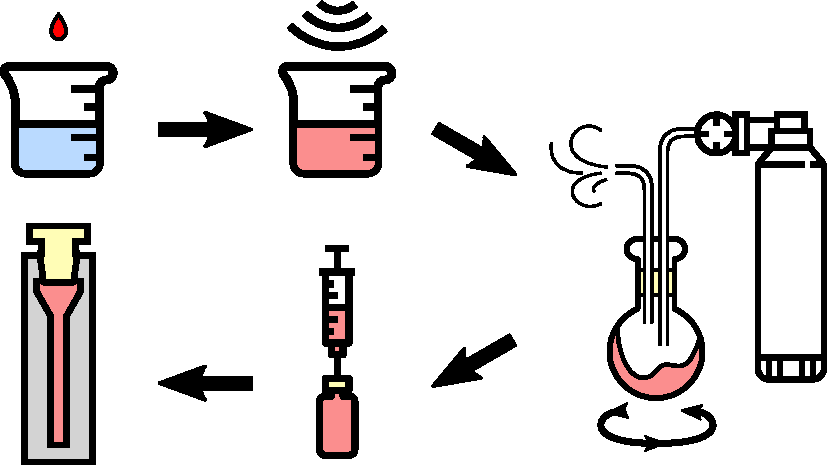
\includegraphics[width=0.95\linewidth]{1_main_matter/co2hb_figures/mes_chain.pdf}
	\caption[Haemolysate preparation, from the vein to the spectrophotometer.]{Haemolysate preparation, from the vein to the spectrophotometer. The different steps are (from top left to bottom left): venous sampling and dilution, ultrasound lysis, tonometry with \gls{co2} or \gls{n2}, careful anaerobic handling, and pouring into airtight glass cuvettes for spectrophotometric measurements.}
	\label{fig:co2hb:co2hb_mes_chain}
\end{figure}

Figure~\ref{fig:co2hb:co2hb_mes_chain} summarises the above-described steps, which led to six different mixtures: diluted lysed blood at 1:10 or 1:1000 ratio, equilibrated with \gls{co2}, \gls{n2}, or ambient air. In addition to these six mixtures, the absorption spectra of the dilution medium were also measured: pure---for baseline correction---and with \gls{edta} and sodium metabisulfite (\gls{sobisulf_for}) separately, to assess the influence of these substances on the haemolysates measurements. Indeed, no information about the absorption spectra of sodium metabisulfite or \gls{edta} in solution could be found in the literature. An analysis of the relative variations of the absorption spectrum of the dilution medium with and without sodium metabisulfite and \gls{edta} was thus performed. Concentrations in the intra medium were 6.1~mM for \gls{edta} and 2.0~mM for sodium metabisulfite.

Finally, the influence of the tonometry duration on the obtained spectra was also investigated. Equilibration durations were varied between 30 and 45~min in 3~min steps, all the while measuring the absorbance value of the 759~nm peak of the \gls{co2hb} and \gls{hb} absorption spectra. A Pearson correlation coefficient test was then performed, searching for an influence of the tonometry duration on the so-obtained absorbance values.

\subsubsection{Assessment of pulse carbametry feasibility}

For pulse carbametry to be achievable, one needs that the absorption spectra of \gls{co2hb} and \gls{hb} exhibit \emph{sufficient} differences at accessible wavelengths\footnote{What is meant by \enquote{accessible wavelength} is further discussed in Section~\ref{sect:co2hb:light_pene} and is not developed here.}.
Assessing how much is \emph{sufficient} is a complex task, which may be answered by addressing the following questions in order.
\begin{enumerate}[label=(\alph*)]
	\item Are the measured average spectra computed for \gls{hb} and \gls{co2hb} different?
	\item If they are, is this difference statistically significant?
	\item Does this difference---observed in the laboratory---translate into something actually exploitable in real life setups, where absorption measurements would be affected by:
	\begin{itemize}
		\item[--] additional absorption caused by tissues surrounding the blood vessels,
		\item[--] light reflection and scattering in the said tissues,
		\item[--] inter-subject variations in physiology,
		\item[--] noises related to ambulatory measurement setups (ambient light, motion),
		\item[--] the accuracy of embedded sensors, which is bound to be lower than that of laboratory spectrophotometers.
	\end{itemize}
\end{enumerate}

Different methods were developed to answer each of these questions, as detailed below.

\subsubsection*{(a) Comparison of average spectra for Hb and \texorpdfstring{CO\(_2\)Hb}{CO2Hb}}

After offset correction and outlier removal, a set of spectra for each haemoglobin species was obtained.
Each of these sets was then averaged to obtain the final absorption spectrum of the corresponding haemoglobin species.
Resulting average spectra were then plotted for visual comparison (see Figure~\ref{fig:co2hb:splitted_hb}).

\subsubsection*{(b) Statistical significance of the difference between spectra}

The problem of assessing whether two absorption spectra are statistically different is non trivial. Indeed, one has to deal with limitations of two kinds:
\begin{enumerate}
	\item The estimated absorption spectrum of each haemoglobin species is a vector of dependent random variables $\hat{A}_\text{species}(\lambda)$ such that
	\begin{equation}
		\forall \lambda,\ \hat{A}_\text{species}(\lambda) \sim \mathcal{N}\left(A_\text{species}(\lambda),\sigma_\text{species}(\lambda)^2\right)
	\end{equation}
	where $\sigma_\text{species}(\lambda)$ is the standard variation of the noise on the measurement of the absorption of the haemoglobin species under consideration at wavelength $\lambda$. Thus, deciding whether the difference in the measured spectra of \gls{hb} and \gls{co2hb} is statistically significant is actually a multivariate analysis problem. Solving the latter would need one to perform at least as many measurements as there are wavelengths in the measured spectra (i.e. several hundreds)\cite{rencher2002}.
	\item Variations in the measured spectrum of each species are bound to be induced by the slight differences in the manipulations specific to each species; thus, a statistically significant difference between measured spectra could actually reveal a difference in the haemoglobin species obtention protocol and not in the absorption spectra themselves.
\end{enumerate}

To address such difficulties, the following analysis was performed on the measured haemoglobin spectra: for both the (\gls{hb},\gls{co2hb}) and (\gls{hb},\gls{o2hb}) pairs of haemoglobin species, we computed the average, minimum, and maximum relative difference of their absorption spectra. This difference, computed for each wavelength, allows one to assess whether there is an exploitable discrepancy between the spectra of \gls{hb} and \gls{co2hb} in the same order of magnitude as that between \gls{hb} and \gls{o2hb}.

\subsubsection*{(c) Applicability in real life setups}\label{sect:co2hb:pulse_carb_feas}

In order to estimate how much difference should be measured between the spectra of \gls{hb} and \gls{co2hb} for it to be exploitable in a pulse carbametry context, parallels were drawn with pulse oximetry. Specifically, it was proposed to:
\begin{enumerate}[label=\textit{(\roman*)}]
	\item use the literature available on pulse oximetry to obtain an estimation of the accuracy of photoplethysmographic measurements on human skin,
	\item derive a theoretical background for pulse carbametry, and
	\item use the afore-mentioned accuracy in such background along with the results of our measurements, to conclude on the feasibility of pulse carbametry.
\end{enumerate}

Note that the analysis presented in the remainder of this chapter is based on a two-wavelengths approach. Even though we acknowledge that multi-wavelengths approaches can improve the performance of photoplethysmographic systems---as above-mentioned in Section \ref{sect:co2hb:spo2_multiwl}---the goal of this study was to evaluate whether there are couples of wavelengths for which the \gls{hb} and \gls{co2hb} absorption spectra exhibit exploitable difference. The optimization of the exploitation of these pairs of wavelengths---should they exist---using a multi-wavelengths approach is thus out of the scope of this study.

\paragraph{\textit{(i)} Accuracy in pulse oximetry} ~\\

Our goal here is not to dive deeply into the theoretical foundations of pulse oximetry---as it has already been done in Section~\ref{sect:co2hb:pulse_oximetry}---but to estimate the sources of inaccuracy of this technique. In pulse oximetry, as mentioned above, the \gls{spo2} is derived from the so-called \emph{ratio of ratio}, $R$, which in turns utilises absorbance of light by human tissues at two different wavelengths. $R$ is given by (Equation~\ref{eq:co2hb:rr_defsao2}):
\begin{equation}\label{eq:co2hb:rr_defspo2}
	R= \frac{\text{\gls{o2sat}} \cdot \varepsilon_{\lambda_1,\text{\gls{o2hb}}} + (1-\text{\gls{o2sat}})\cdot \varepsilon_{\lambda_1,\text{\gls{hb}}}}{\text{\gls{o2sat}} \cdot \varepsilon_{\lambda_2,\text{\gls{o2hb}}} + (1-\text{\gls{o2sat}})\cdot \varepsilon_{\lambda_2,\text{\gls{hb}}}}
\end{equation}
where $\lambda_1$ and $\lambda_2$ are the two measurement wavelengths, often 660~nm and 940~nm, and $\varepsilon_{\lambda_i, X}$ are the haemoglobin extinction coefficients of the $X$ haemoglobin species at wavelength $\lambda_i$.

The question at stake for addressing \textit{(i)} is then: what accuracy on $R$ is achievable in practice by common photoplethysmographic sensors? As can be seen from Equation~\ref{eq:co2hb:rr_defspo2}, such an accuracy on $R$ can be estimated based on the accuracy on the \gls{o2sat} that is reported in the literature. The latter has been studied in many clinical trials---themselves reviewed\cite{nitzan2014, jubran2015}---and a mean standard deviation of 2\% on the 70\%--100\% \gls{o2sat} range can be considered to be achievable under good measurement conditions---that is, mainly no movement from the subject and a good perfusion index. Figure~\ref{fig:oxy_acc} represents the results obtained when taking such a standard deviation for \gls{o2sat} and computing the corresponding $R$ measurement inaccuracies at the 660~nm and 940~nm wavelengths---the two most-used wavelengths in pulse oximetry---using Zijlstra \etal{}\cite{zijlstra2000} absorption coefficient for \gls{o2hb} and \gls{hb}.

\begin{figure}
	\centering
	\includegraphics{1_main_matter/co2hb_figures/tikz/out/oxy_rr_anal.pdf}
	\caption[Pulse oximetry ratio of ratios error]{\textbf{Left}: an error of 2\% on the \gls{o2sat} reading at 80\% of \gls{o2sat} (in blue), is the result of an inaccuracy of 6.7\% on the measurement of $R$ (in red). \textbf{Right:} conversely, if we impose a 2\% error on the \gls{o2sat} reading, we can compute the relative variation of $R$ which generated such error. Again, at 80\% \gls{o2sat}, the latter is 6.7\% (dashed black lines).}
	\label{fig:oxy_acc}
\end{figure}

One can see that the lower the oxygen saturation is, the more accurate the measurement of $R$ needs to be to guarantee a given accuracy on \gls{o2sat}. Indeed, while the accuracy on $R$ measurement must be as low as 5.6~\% at 70~\% of \gls{o2sat}, it can be as high as 13.3\% at 98~\% of \gls{o2sat}. Of note, such calculations were made with the hypothesis that all errors were following Gaussian distributions.

\paragraph{\textit{(ii)} Accuracy in pulse carbametry}

This minimum error---5.6\%---derived in the case of pulse oximetry gives a best-case---hence optimistic---value of the achievable accuracy on $R$ measurement using transcutaneous ratiometric techniques. When applying a similar method to obtain the concentration of \gls{co2hb} in arterial blood using pulse carbametry, one may thus expect---at best---a similar accuracy on $R$ estimation. The pulse carbametry context considered in this study is detailed in the remainder of this paragraph.

Let us consider a binary system composed solely of \gls{hb} and \gls{co2hb} and define the \gls{co2sat} as:

\begin{equation}
	\text{\gls{co2sat}} = \frac{ [\text{\gls{co2hb}}] }
	{ [\text{\gls{co2hb}}] + [\text{\gls{hb}}]}
\end{equation}

Wherein [\gls{hb}] and [\gls{co2hb}] are the \gls{hb} and \gls{co2hb} concentrations, respectively. Using the pulse oximetry theoretical background---see Section \ref{sect:co2hb:pulse_oximetry}---\gls{co2sat} can be derived from a measured ratio of ratio $R$ as:

\begin{equation}\label{eq:co2sat_exp}
	\text{\gls{co2sat}}(\lambda_1,\lambda_2) = \frac{\varepsilon_{\lambda_1, \text{\gls{hb}}} - R \cdot \varepsilon_{\lambda_2, \text{\gls{hb}}}}
	{(\varepsilon_{\lambda_1, \text{\gls{hb}}} - \varepsilon_{\lambda_1, \text{\gls{co2hb}}}) - R\cdot (\varepsilon_{\lambda_2, \text{\gls{hb}}} - \varepsilon_{\lambda_2, \text{\gls{co2hb}}} )}
\end{equation}

The feasibility of pulse carbametry will be assessed as follow: considering the extinction coefficients $\varepsilon_{\text{\gls{co2hb}}}$ and $\varepsilon_{\text{\gls{hb}}}$ derived from our spectrophotometric measurements, and the afore-mentioned standard deviation on $R$, the standard deviation on \gls{co2sat} will be computed for each ($\lambda_1$,$\lambda_2$) couple on the 235--1000~nm range. Then, finding the minimum value of this deviation with respect to ($\lambda_1$,$\lambda_2$) will provide the best achievable accuracy using pulse carbametry. More explicitly, the minimum \gls{co2sat} accuracy reachable with pulse carbametry is given by:

\begin{equation}\label{eq:co2sat_err}
	\delta\text{\gls{co2sat}} = \min_{(\lambda_1,\lambda_2)} \sigma\text{\gls{co2sat}}(\lambda_1,\lambda_2)
\end{equation}

Wherein $\sigma\text{\gls{co2sat}}(\lambda_1,\lambda_2)$ is the relative standard deviation of $\text{\gls{co2sat}}(\lambda_1,\lambda_2)$, computed from the $R$ standard deviation in the case of pulse oximetry (5.6\%). Judging whether a given minimal accuracy $\delta\text{\gls{co2sat}}$ is \emph{small enough} is essentially an arbitrary choice. Still, one can rely on the clinically accepted range for \gls{paco2}, which is $\pm$7.5~mmHg (95\% limits of agreement, corresponding to $\pm$2~S.D.)\cite{bendjelid2005}. This latter range translates into a standard deviation of 9\% on \gls{paco2} reading, at a standard \gls{paco2} level of 40~mmHg. Thus, the decision threshold on $\delta\text{\gls{co2sat}}$ was set to this value as a first approximation, \ie{} if $\delta\text{\gls{co2sat}}$ is below 9\%, pulse carbametry will be considered feasible.

\subsection{Results}

\subsubsection{Haemoglobin spectra}\label{sect:co2hb:hb_spectra}

The obtained spectra of diluted lysed blood equilibrated with ambient air, pure \gls{n2} and pure \gls{co2} are presented in Figure~\ref{fig:co2hb:splitted_hb} after baseline correction and outlier removal. Each spectrum was averaged over (UV-Vis/Vis-IR spectra number): 24/13 (\gls{co2}), 10/17 (\gls{n2}) and 32/38 (air) measurements. The variations in the number of trials between the different gases are explained by several factors. At first, there were two different measurement campaigns for the UV-Vis and Vis-IR range, leading to less measurements in the Vis-IR (some fluorescence measurements were performed instead, see Section \ref{sect:co2hb:fluo}). Then, there were twice as much measurements made with {\gls{o2hb}} as with {\gls{n2}} or {\gls{co2}}, only because {\gls{o2hb}} was readily available and measured while waiting for {\gls{hb}} and {\gls{co2hb}} to be obtained by tonometry. Finally, an outlier removal algorithm based on the standard deviation of the measurements was used, removing measurements diverging more than roughly {$\pm$}2.5 standard deviation from the mean, using an adaptative threshold and a recursive algorithm inspired by the work of Hadi \textit{et al.}{\cite{hadi1992}}---see Appendix~\ref{app:pruning_algo}. This threshold choice was arbitrary, as is that of outlier detection and removal in the general case{\cite{aguinis2013}}. Given the important number of wavelengths in each measurement and the limited number of measurements performed, a power calculation was not feasible.

\begin{figure}
	\centering
		\includegraphics{1_main_matter/co2hb_figures/tikz/out/splitted_hb.pdf}
	\caption[Measured absorption spectra of diluted lysed blood tonometered with \gls{o2}, \gls{n2} or \gls{co2}]{Measured absorption spectra of diluted lysed blood tonometered with \gls{o2}, \gls{n2} or \gls{co2}. The vertical scale is arbitrary, data were scaled for representation and corresponds to two different dilution ratios of 1:1000 for the UV-Vis 235--600~nm range (left) and 1:10 for the Vis-IR 600--1000~nm range (right) (ranges are 235--590~nm and 590--1000~nm for air--equilibrated solutions). The black dashed line separates the UV-Vis from the Vis-IR measurements.}
	\label{fig:co2hb:splitted_hb}
\end{figure}

The absorption spectra of \gls{hb} and \gls{co2hb} appear to be extremely close, especially compared to \mbox{\gls{o2hb}}. The standard deviations in absorption for \gls{o2hb}, \gls{co2hb} and \gls{hb} were (mean standard deviation, mininum, maximum) 1.20$\substack{7.55 \\ 0.38}$~mAbs, 3.16$\substack{36.34 \\ 0.51}$~mAbs and 2.43$\substack{21.02 \\ 0.40}$~mAbs, corresponding to relative variations of 0.53$\substack{2.24 \\ 0.14}$\%, 1.08$\substack{5.74 \\ 0.05}$\% and 0.81$\substack{4.59 \\ 0.07}$\%, respectively.

% /!\ PERCENT est invariable en anglais
Figure \ref{fig:co2hb:var_analysis} gives a more quantitative analysis to the difference between \gls{o2hb}, \gls{co2hb} and \gls{hb} spectra. While the relative differences between \gls{o2hb} and \gls{hb} spectra---clearly visible in Figure~\ref{fig:co2hb:splitted_hb}---can reach several tens of percent, those between \gls{co2hb} and \gls{hb} are much more tenuous. The differences between mean \gls{o2hb} and \gls{hb} spectra on the one hand and \gls{co2hb} and \gls{hb} spectra on the other hand were (mean absolute difference, maximum) 0.18$\substack{(1.99) \\ {} }$~Abs and 0.08$\substack{(0.11) \\ {}}$~Abs, corresponding to relative variations of 36$\substack{(153) \\ {}}$\% and 2$\substack{(13) \\ {}}$\%, respectively.

\begin{figure}
	\centering
	\includegraphics{1_main_matter/co2hb_figures/tikz/out/var_analysis}
	\caption[Relative differences between \gls{hb} / \gls{co2hb} and \gls{hb} / \gls{o2hb} absorption spectra.]{Relative differences between \gls{hb} and \gls{co2hb} (in blue) and between \gls{hb} and \gls{o2hb} (in red) absorption spectra. The two thin lines for each comparison represent the maximum and minimum values along all measurements. For instance, for the \gls{hb} / \gls{co2hb} comparison at a given wavelength, the higher line represents \gls{hb} maximum value minus \gls{co2hb} minimum value, while the lower line represents \gls{hb} minimum value minus \gls{co2hb} maximum value (both normalised by \gls{co2hb} mean value).}
	\label{fig:co2hb:var_analysis}
\end{figure}

\subsubsection{Intra medium}

Figure~\ref{fig:co2hb:dilution_full} presents absorption spectra of the dilution medium with and without sodium metabisulfite. Results with \gls{edta} are not shown since they were indistinguishable from pure dilution medium on a full scale view. More subtle effects of these substances are shown in Figure~\ref{fig:co2hb:dilution_err}, which focuses on the relative deviations of the prepared \gls{edta} or sodium metabisulfite solutions with respect to pure dilution medium. Again, each spectrum is averaged over several measurements: 28/34 (pure) and 12/11 (sodium metabisulfite) measurements for the UV-Vis/Vis-IR range, and 5 (\gls{edta}) measurements for the Vis-IR only range.

\begin{figure}
	\centering
	\includegraphics{1_main_matter/co2hb_figures/tikz/out/dilution_full}
	\caption[Absorption spectra of the dilution medium with and without sodium metabisulfite.]{Absorption spectra of the dilution medium with and without the addition of sodium metabisulfite (2.0~mM). Note the marked absorption of sodium metabisulfite in the ultraviolet, up to almost 500~nm.}
	\label{fig:co2hb:dilution_full}
\end{figure}

\begin{figure}
	\centering
	\includegraphics{1_main_matter/co2hb_figures/tikz/out/dilution_rel_error}
	\caption[Relative variations of the dilution medium absorption spectrum with sodium metabisulfite and \gls{edta}.]{Relative variations of the dilution medium absorption spectrum upon the addition of \gls{edta} (0.61~mM) or sodium metabisulfite (2.0~mM). The left side is multiplied by 0.1 ($\sim$10\% of relative variation for sodium metabisulfite at 500~nm). Of note, the slightly negative values in the 575--600~nm range are likely to be measurement artefacts due to measurements in the lower sensitivity limit of the spectrophotometer, given the measurements presented in Figure~\ref{fig:co2hb:dilution_full} and the relative variation above 4\% just above 600~nm.}
	\label{fig:co2hb:dilution_err}
\end{figure}

\subsubsection{Tonometry duration}\label{sect:co2hb:tonodur}

The influence of tonometry duration on the measured absorbances was found to be insignificant for durations between 30 and 45~min, with test results being {$\rho$}=-0.13, {$p$}=0.62, on 17 samples for {\gls{n2}} tonometry and {$\rho$}=-0.04, {$p$}=0.91, on 13 samples for {\gls{co2}} tonometry (Pearson correlation coefficient). It was thus concluded that 30~min of equilibration time were enough to obtain either {\gls{co2hb}} or {\gls{hb}}.

\subsubsection{Pulse carbametry}

The \gls{co2hb} and \gls{hb} absorption spectra presented in Figure~\ref{fig:co2hb:splitted_hb}---and obtained through \gls{co2} and \gls{n2} tonometry, respectively---were then used to perform the analysis presented in Section~\ref{sect:co2hb:pulse_carb_feas}. The value of $\sigma\text{\gls{co2sat}}$ as a function of the two wavelengths $(\lambda_1, \lambda_2)$ are shown in Figure~\ref{fig:co2hb:satco2_err}.

\begin{figure}
	\centering
	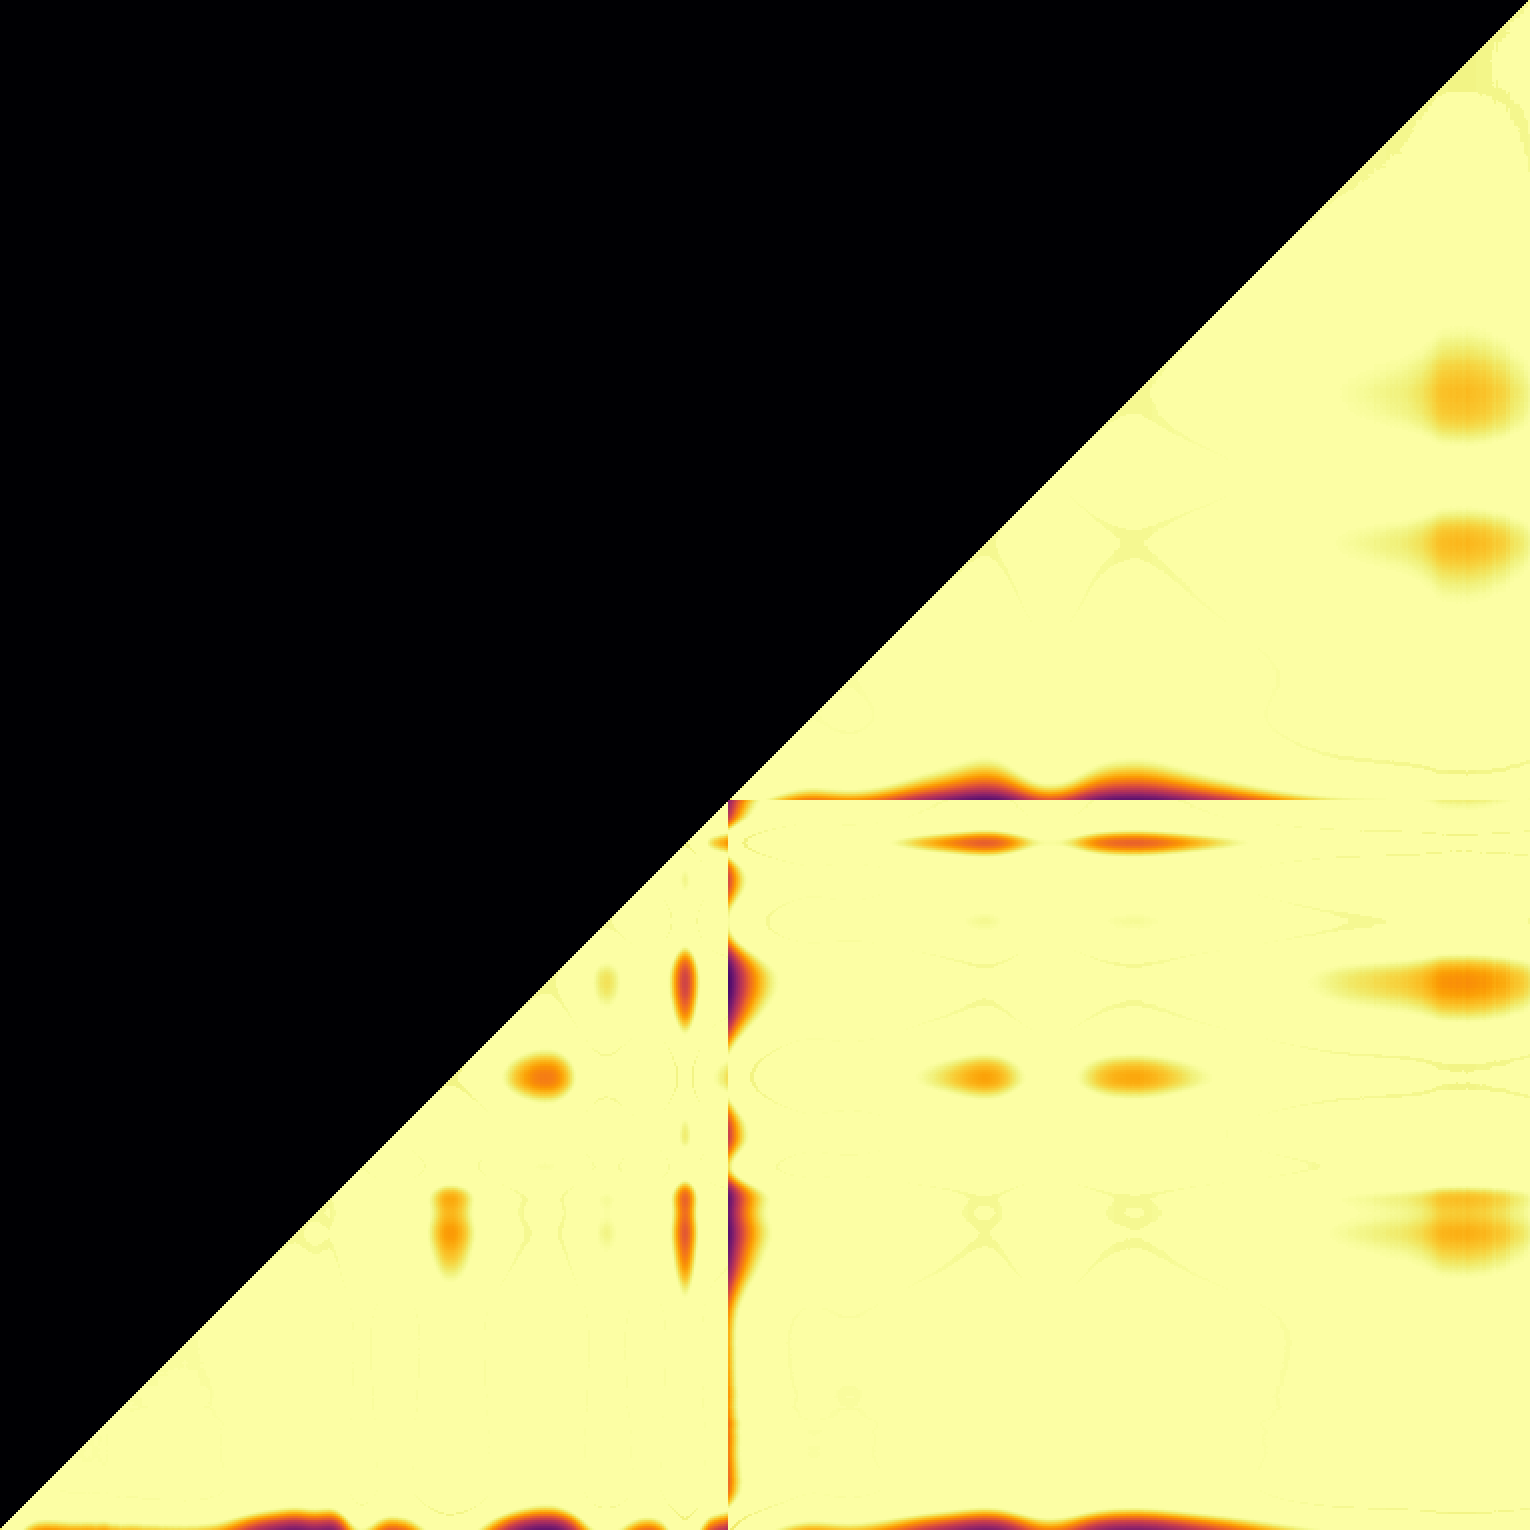
\includegraphics{1_main_matter/co2hb_figures/tikz/out/co2sat_heatmap}
	\caption{$\sigma\text{\gls{co2sat}}$ as a function of $(\lambda_1, \lambda_2)$ on the 235--1000~nm range.}
	\label{fig:co2hb:satco2_err}
\end{figure}

The minimal value taken by $\sigma\text{\gls{co2sat}}$, is $\delta\text{\gls{co2sat}} = 34.2\%$ at $\lambda_1$ = 508~nm and $\lambda_2$ = 600~nm. However, as can be seen from the asymmetry of the spots on the $\lambda_1$=600~nm or $\lambda_2$=600~nm lines, these values likely originates from limitations of the measurement system that was used. Indeed, when using a 1:1000 dilution ratio, the lysed blood absorbance was below 1.2~Abs on the full 235--600~nm range, which is acceptable. At the opposite, when a 1:10 dilution ratio was used, the latter absorbance topped at 2.8~Abs near 600~nm, which is close to the saturation value of 3.0~Abs of the used spectrophotometer. Ideally, to circumvent this flaw of the measurement setup, three dilutions at 1:10, 1:100 and 1:1000 should have been performed on the 235--450~nm, 450--650~nm and 650--1000~nm ranges respectively.

Still, even with these flaws, which---in the worst case---could increase the spectral differences between \gls{hb} and \gls{co2hb} and thus lower the error on \gls{co2sat} measurements, the reached accuracy is still far above the 9\% target established previously. If $\sigma$\gls{co2sat} values near the 600~nm lines are discarded and focus is made on other spots---such as the ($\lambda_1$=510~nm, $\lambda_2$=580~nm) area---values above 41\% are to be found for $\delta$\gls{co2sat}.

\subsection{Discussion}

At first, the chosen method for obtaining \gls{co2hb}, \gls{hb} and \gls{o2hb} is discussed. Then the haemoglobin spectra are compared with those available in the literature, the influence of \gls{edta} and sodium metabisulfite is also discussed. Finally, the feasibility of pulse carbametry is assessed.

\subsubsection{On the chosen method}

Among the several authors who measured haemoglobin absorption spectra, some used freshly drawn blood\cite{horecker1943, barlow1962, assendelft1970, mook1979, wray1988, mendelson1989, cope1991, zijlstra1991, zijlstra2000, mieczkowska2011} whereas others preferred lyophilised haemoglobin\cite{drabkin1935, dalziel1957, robles2010}. Lyophilised blood, despite its convenience, has several drawbacks. First, it is composed merely of \gls{methb}\cite{sigma7379, mieczkowska2011} and thus needs an oxidation procedure to convert it back into \gls{o2hb}, a step which involves chemicals that might interfere with the haemoglobin spectrum. Second, a better affinity of haemoglobin has been reported for haemoglobin extracted from freshly drawn blood\cite{horecker1943, mieczkowska2011}. These considerations drove our choice towards fresh blood as a haemoglobin source.

However, fresh blood requires the lysis of erythrocytes and other blood cells to yield a limpid solution. Despite the common use of a surfactant such as Sterox SE\cite{assendelft1970, mook1979, zijlstra1991} or equivalent\cite{horecker1943, wray1988, cope1991}, we preferred an ultrasound lysis, which adds no foreign chemical in blood for the same effect\cite{mendelson1989}. Fresh blood sampling could also require centrifugation in order to keep only the erythrocytes and avoid spectral interferences from other blood components, namely leucocytes and lipids. Yet, since haemoglobin is the main absorbing compound in blood by two up to three orders of magnitude\cite{meinke2007}, we did not consider the centrifugation step mandatory. Lastly, fresh blood sampling requires the addition of an anticoagulant if it is not largely diluted. Consequently, for the 1:10 dilution ratio---on the 600--1000~nm range---we considered the addition of \gls{edta} to the collected blood. The spectral influence of the latter was measured, and found to be negligible on the studied range---as shown in Figure~\ref{fig:co2hb:dilution_err}---with relative absorption variations in the $\pm$1\% range, corresponding to absolute variations in the $\pm$1~mAbs range, well below the measured standard deviation on the absorption spectrum of the dilution medium (1.24$\substack{+14.1 \\ -9.3}$~mAbs for the dilution medium alone, for instance, and similar values were found for the dilution medium with 2.0~mM \gls{edta}). We concluded that \gls{edta} did not have any influence on the measured spectra in the quantity used in our experiments.

Concerning haemoglobin measurements in its reduced form, the use of sodium dithionite (\gls{sodith_for}) has been reported as a mean to quickly obtain \gls{hb}\cite{barlow1962, assendelft1970, mendelson1989, robles2010, mieczkowska2011}. Alas, it has also been reported to alter the absorption spectrum of the latter\cite{dalziel1957, schubart1957, zijlstra2000}. We conducted investigations on the possible use of sodium metabisulfite (\gls{sobisulf_for}) which---like sodium dithionite---leads in aqueous solution to the production of bisulfite anions (\ce{HSO_3^-}), the strong reducing agent converting \gls{o2hb} into \gls{hb}. Our results---see Figure~\ref{fig:co2hb:dilution_full} and \ref{fig:co2hb:dilution_err}---confirm earlier observations and extend them with quantitative measurements on the 235--1000~nm range. Because of this, we would not recommend the use of bisulfite anions for their strong absorption, particularly at short wavelengths up to 500~nm.

Tonometry was thus chosen for the obtention of \gls{hb} and \gls{co2hb} to avoid using the afore-mentioned reducing agents. Concerning its duration, 30~min were found to be sufficient in spherical glass tonometers filled with 6~mL of diluted lysed blood, as demonstrated in Section~\ref{sect:co2hb:tonodur}. However, one should bear in mind that this duration is strongly dependant on several parameters, such as the shape of the tonometer used for equilibration, its filling level, or the gas flow rate, for instance.

The dilution medium was chosen in order to correspond to an intracellular medium (with high K$^+$ concentration). pH was also set to an erythrocyte intracellular value of 7.2 since it has been reported to be that of the inner erythrocytes\cite{jensen2004, kummerow2000}. It has also been reported that pH has an impact---although relatively small---on the measured haemoglobin spectra\cite{dalziel1957, wimberley1988, zijlstra1997}. Concerning the choice of HEPES as a buffer, a better preservation of the haemoglobin oxygenation function was reported with HEPES over Tris/Bis-Tris\cite{weber1992}. Finally, the chosen dilution ratios are justified since haemoglobin has been reported to follow Beer-Lambert law, would it be for extremely diluted or concentrated solutions\cite{drabkin1935}.

\subsubsection{Haemoglobin spectra}

The measured spectra of diluted lysed blood, either equilibrated with \gls{n2} or ambient air, are extremely close to that of the literature for \gls{hb} and \gls{o2hb}, as can be seen on Fig. \ref{fig:co2hb:compiled_spectra}. This comforts us in the method that we employed and the above-mentioned choices. The small discrepancies observed between our spectra and that of the literature may be explained by a number of methodological differences. For instance, several authors\cite{assendelft1970, mook1979, zijlstra1991} used a surfactant such as Sterox SE to perform the erythrocyte lysis, while we chose to use ultrasounds. The surfactant may have a spectral impact, which---to the best of our knowledge---has never been quantified. Other authors, even when choosing tonometry, added some small amount of sodium dithionite before measuring\cite{zijlstra2000}. Yet, sodium dithionite, like sodium metabisulfite, is known to have a marked spectral influence\cite{dalziel1957}. Zijlstra \etal{}\cite{zijlstra2000} also mentioned that in case of too long tonometry, supernatant residues sometimes appeared in the diluted blood, the nature of which was not determined. Although we did not observe such behaviour, a small turbidity might have been present in their measurements, or ours. Among the literature spectra presented in Figure~\ref{fig:co2hb:compiled_spectra}, while Assendelft, and Zijlstra detailed their protocol, Prahl and Kolyva only offer raw coefficients. It is therefore difficult to analyse the potential sources of differences between their spectra, or between their spectra and ours.

\begin{figure}
	\centering
	\includegraphics[width=0.95\linewidth]{1_main_matter/co2hb_figures/tikz/out/compiled_spectra}
	\caption[Obtained haemoglobin spectra: comparison with the literature.]{Our measurements (plain line) compared to that of Prahl\cite{prahl1998}, Zijlstra \etal\cite{zijlstra2000}, Kolyva \etal\cite{kolyva2012} and Assendelft\cite{assendelft1970}. Our measurements are consistent with that of the literature for \gls{o2hb} (Air) and \gls{hb} (\gls{n2}).}
	\label{fig:co2hb:compiled_spectra}
\end{figure}

Overall, the repeatability of the measurements was fairly good, with mean standard deviation of 0.53\%, 1.08\% and 0.81\%, for \gls{o2hb}, \gls{co2hb} and \gls{hb} measurements, respectively, which can be compared to values between 0.4\% and 2.1\% reported by Zijlstra \etal{} for various haemoglobin species\cite[Table~8.3]{zijlstra2000}. The rather high maximum standard deviations reported in Section~\ref{sect:co2hb:hb_spectra} (2.24\%, 5.74\% and 4.59\% for \gls{o2hb}, \gls{co2hb} and \gls{hb}, respectively) are mainly due to the measurement limits of the spectrophotometer near 600~nm, corresponding to either too low ($\leq$0.05~Abs) absorbance below 600~nm, or too high ($\geq$2.5~Abs) absorbance above 600~nm. When computing the mean standard deviation without the 580--620~nm range for \gls{o2hb}, \gls{co2hb} and \gls{hb}, maximum standard deviations values drop to 7.25~mAbs, 12.60~mAbs and 21.02~mAbs, corresponding to relative variations of 1.31\%, 2.78\% and 2.54\%, respectively. The mean absorption spectra that we measured for {\gls{o2hb}}, {\gls{co2hb}} and {\gls{hb}} were published as a supplementary material with this original publication\cite{dervieux2020}.

Unfortunately for the future of pulse carbametry, Figure~\ref{fig:co2hb:splitted_hb} also reveals that the absorption spectra of \gls{hb} and \gls{co2hb} are extremely close, their differences being more than one order of magnitude below the ones between the \gls{o2hb} and \gls{hb} absorption spectra, as can be seen of Figure~\ref{fig:co2hb:var_analysis}. Moreover, the measured \gls{hb} and \gls{co2hb} spectra are similar to the \gls{hb} spectra already available in the literature, as can be seen in Figure~\ref{fig:co2hb:compiled_spectra}. Such observations tends to make one believe that the formation of carbamate compounds between \gls{co2} and haemoglobin terminal amine groups does not change the haemoglobin molecule conformation significantly, hence bringing no spectral alteration. However, such intuition shall not have the value of evidence, this is why the possible use of slight differences between \gls{hb} and \gls{co2hb} will now be discussed.

\subsubsection{Pulse carbametry}

Given the 9\% accuracy threshold that was fixed for $\delta$\gls{co2sat}, and the observed value of 34.2\%---or even more if the values close to the spectrophotometer saturation limit are discarded---we could readily conclude that pulse carbametry---as it was presented---is not feasible. However, several additional aspects of this technique need to be further discussed.

At first sight, the consideration of a binary system composed solely of \gls{hb} and \gls{co2hb} can seem surprising. Indeed, in practice, human arterial blood is composed at least of \gls{o2hb}, \gls{hb} and \gls{co2hb}---and even \gls{cohb}\cite{mcilvaine1969, wald1981} and \gls{methb}\cite{kravitz1956, vankampen1966} in small amounts. That being said, it should be clear that the demonstrated inability to distinguish between \gls{co2hb} and \gls{hb}, even when they are the only absorbing compounds involved, would be worsened by the addition of any other perturbing absorbing species---\eg{} \gls{o2hb}. An in-depth analysis of the tertiary system \gls{o2hb}--\gls{hb}--\gls{co2hb} would have been necessary only if pulse carbametry had been found to be possible in a binary system.

Then, we made the hypothesis that all studied errors were Gaussian. It is most often considered to be the case in the literature\cite{nitzan2014, jubran2015} and we also stuck to this hypothesis in the absence of evidence to the contrary. Thus, the main remaining question is to know whether the mathematical functions giving $R = f(\text{\gls{o2sat}})$ and $\text{\gls{co2sat}} = g(R)$ can be reasonably linearly approximated. The latter assumption has to be checked for $f$ at the 660/940~nm couple, and for $g$ on the full 235--1000~nm range. The calculation of the derivative of these two functions is straightforward and allows one to conclude that the relative variation of the slope of $f$ stays below 3.8\% on the 70--100\% \gls{o2sat} range at 660/940~nm, whereas the slope of $g$ stays below 2.2\% on the 0--100\% \gls{co2sat} range at 340/600~nm (maximal value on the 235--1000~nm range). We can thus safely conclude that approximating $f$ and $g$ with linear functions is reasonable and that our hypothesis concerning Gaussian errors is justified.

Next, all the calculations leading to Figure~\ref{fig:co2hb:satco2_err} were made considering a monochromatic skin illumination. In a typical pulse carbametry application, the light source is more likely to be a laser, laser diode, or \gls{led}. In such cases---and especially when using an \gls{led}---the effect of a non monochromatic light source will be a degradation of $\delta$\gls{co2sat} caused by the spectral spread of the source. Such spread will basically smooth the \gls{hb} and \gls{co2hb} absorption spectra by convolving them with the emission spectrum of the source. The latter can in turn be regarded as a roughly Gaussian window of \gls{fwhm} of a few (laser sources) or a few tens (\gls{led}) of nanometres. For instance, a source with a \gls{fwhm} of 5~nm leads to a $\delta$\gls{co2sat} of 36.8\%; with a \gls{fwhm} of 20~nm this value reaches 42.1\%, to be compared with the 34.2\% of the aforementioned ideal monochromatic case.

Finally, the last assumption that we made concerns the extrapolation to pulse carbametry of the accuracy on $R$ measurement in the \gls{o2sat} case. Such an assumption was made considering that the 660~nm and 940~nm wavelengths were not chosen randomly but to maximize pulse oximetry sensitivity. In other words, they were chosen such that a small change in \gls{o2sat} translates into a huge change in measured light intensity at certain wavelengths\cite{mook1969, assendelft1970}, but also such that they were in the tissues \emph{optical window}---the 700--1000~nm range\cite{wilson1985, melo2001, ash2017}. Such considerations make the \gls{o2sat} 660/940~nm situation a best case, and we would expect other wavelengths couples to give equally or worse accurate $R$ measurements. This remains, however, a supposition since---to the best of our knowledge---there appears to be only a few studies on the measurement accuracy on \gls{o2sat}---and thus $R$---at wavelengths different from the usual 660/940~nm pair (see Section~\ref{sect:co2hb:spo2_multiwl}). Still, it is worth noticing that our conclusions would remain unchanged, even if we managed somehow to drastically reduce the measuring accuracy on $R$---say by a factor two or three, we would still have a $\delta$\gls{co2sat} value above 9\%.

\subsection{Conclusion}

In the afore-presented study, the \gls{co2hb} absorption spectrum was measured for the first time. \gls{o2hb}, \gls{hb} and \gls{co2hb} were obtained from diluted lysed blood equilibrated with ambient air, pure \gls{n2} and pure \gls{co2} respectively. The methodology leading to their obtention and isolation was discussed thoroughly, including the possible use of \gls{edta} or sodium metabisulfite.

The absorption spectra of \gls{o2hb} and \gls{hb} were close to that of literature, while the absorption spectrum of \gls{co2hb} was extremely close to that of \gls{hb}. No influence of \gls{edta} was found, whereas sodium metabisulfite---on the contrary---strongly absorbs in the ultraviolet and visible range up to 500~nm. As such, the latter should not be used in this spectral range for haemoglobin reduction.

A theoretical variation of pulse oximetry applied to the determination of \gls{co2hb} fraction was presented, which we called pulse carbametry. This theoretical framework was applied to the afore-mentioned measurements to conclude whether the slight variations observed between the \gls{hb} and \gls{co2hb} absorption spectra could be used in such context. Our observations show that such approach seems extremely challenging since these spectra are almost identical. In particular, on the basis of current knowledge, pulse carbametry may not be used in medical practice.

Yet, the present work may benefit from further investigations to consolidate its conclusions. In particular, only two wavelengths were considered for pulse carbametry. It would be interesting to use more sophisticated multi-wavelengths approaches, since they usually give better results in the case of pulse oximetry\cite{katja2011}, although the question of wavelengths selection becomes more complex\cite{brunelle1996, brendel2009}.

\section{Additional Fluorescence Measurement}\label{sect:co2hb:fluo}

\subsection{Introduction}

Following the negative results of the previous section, I decided to also investigate haemoglobin fluorescence properties to be on the safe side. Fluorescence is a long-known optical method for the characterization of chemicals. Its basic principle is to illuminate an analyte at a given wavelength, and to measure the light re-emitted by the sample under study. A fluorescent material will absorb photons at the excitation wavelength and re-emit photons at the same wavelength (Rayleigh scattering), at a greater wavelength (Stokes shift or Stokes Raman scattering), or at a smaller wavelength (anti-Stokes shift, anti-Stokes Raman scattering). For more information on the fluorescence phenomenon itself, I kindly redirect the curious reader towards the first chapters of the excellent \textit{Molecular Fluorescence: Principles and Applications} book, by Bernard Valeur \etal{}\cite{valeur2012molecfluo}.

The aim of this section is to evaluate the feasibility of using conventional fluorescence techniques on the human skin, in order to gather information about the oxidation or carbamation status of the haemoglobin contained in the subcutaneous blood. Indeed, haemoglobin has been shown to fluoresce slightly between 300~nm and 400~nm when excited at 280~nm or 296~nm. More interestingly, this fluorescence has been reported to depend on the oxygenation status of the haemoglobin protein\cite{itoh1981, hirsch2003}. In a first part, bibliographic resources of previous work found in the literature about the fluorescence of human haemoglobin, tissues, and more specifically different skin layers, are presented. The feasibility of the aforementioned approach is then discussed in a second part.

\subsection{Previous work}\label{sect:co2hb:fluo:prev_work}

The feasibility of haemoglobin fluorescence measurements through the human skin relies mainly on three requirements. First, the haemoglobin molecule must exhibits a measurable fluorescence. Second, the surrounding medium---predominantly blood and tissues---must not disturb the measurements with the presence of other surrounding endogenous fluorophores. Third, the probed tissues---namely the external layers of the skin in the case of transcutaneous measurements---must be transparent to both the excitation wavelength and the emission wavelength of haemoglobin. These three key points will be discussed in the following subsections.

\subsubsection{A Brief History of Haemoglobin Fluorescence}\label{sect:co2hb:fluo:hb_fluo}

The story begins in 1957 with the discovery by Teale \etal{} of the fluorescence of several aromatic amino acids---namely phenylalanine, tryptophan and tyrosine\cite{teale1957}. These three species exhibit a main excitation peak between 200 and 225~nm and a secondary one between 250 and 290~nm, for fluorescence maxima at 282 (phenylalanine), 303 (tyrosine) and 348~nm (tryptophan). Those three amino acids are of particular interest since they are all present in haemoglobin\footnote{For more information on the haemoglobin structure, see the extensive work of Mitchel Weissbluth on the topic\cite[Table~1.1]{weissbluth1974}, itself based on the discovery of haemoglobin structure using X-rays in the fifties by Nobel prize Max Ferdinand Perutz\cite{perutz1964}.}. The early work of Teale on amino acid was extended in the eighties by several teams---mentioned below---with fluorescence measurements of complete haemoglobin molecules. The difficulty to produce fluorescence spectra for haemoglobin lies in the fact that the molecule itself is a pigment with a very strong absorption in the emission spectrum of its tryptophan constituents. This self-absorbing phenomenon is often referred to as \emph{self quenching}.

Hirsch \etal{} exhibited the existence of a haemoglobin fluorescence attributed to tryptophan in 1980\cite{hirsch1980}. Interestingly, Hirsch noted that above a concentration of 0.16~mM haemoglobin, no further increase in the measured fluorescence could be observed. The given explanation was that above this threshold, more haemoglobin generates more light but also quenches more of the re-emitted light, which leads to an observed fluorescence intensity independent of the haemoglobin concentration above 0.16~mM. Such observations were made possible by the use of front-face optics. Had they used conventional right-angle optics, they would have observed a decreasing fluorescence intensity for higher haemoglobin concentration due to the above mentioned self quenching effect---the interested reader may refer to Appendix~\ref{app:haemo_self_quench} for further explanations on the latter phenomenon. Hirsch's team extended this work in 1981\cite{hirsch1981}, exhibiting a difference of fluorescence between \gls{o2hb} and \gls{hb}. This difference is presented as a consequence of the conformational modification of the haemoglobin from its R (relaxed) to its T (tense) shape\footnote{This is a simplified view of what actually happens, see Yuan \etal{} for more details on the haemoglobin molecule conformational changes\cite{yuan2015}.}, and the corresponding fluorescence spectra are reproduced in Figure~\ref{fig:co2hb:hirsch1981_fluo}.

\begin{figure}
	\centering
	\includegraphics{1_main_matter/co2hb_figures/tikz/out/hirsch_fluo.pdf}
	\caption[Fluorescence emission spectra of adult human haemoglobin in various liganded states.]{Fluorescence emission spectra of adult human haemoglobin in various liganded states---\ie{} \gls{hb}, \gls{o2hb} and \gls{cohb}---uncorrected for baseline. Haemoglobin concentration was 155~\textmu{}M. All measurement were taken in pH~7.35, 50~mM potassium phosphate buffer, at 25{\degree}C. (a): 280~nm excitation; (b): 296~nm excitation. The lower dotted lines are the baselines obtained with the buffer solution alone. Drawn using data from \cite{hirsch1981}.}
	\label{fig:co2hb:hirsch1981_fluo}
\end{figure}

Still in 1980, Alpert \etal{} also used a right-angled fluorometer with extremely diluted haemoglobin solutions (2~\textmu{}M)\cite{alpert1980}. They showed that haemoglobin exhibit a fluorescence similar to that of apohaemoglobin (the polypeptidic chain of haemoglobin without any haeme site) or tryptophan solutions. This attribution of the haemoglobin fluorescence to tryptophan was yet again proposed by Itoh \etal{} in 1981\cite{itoh1981} while measuring fluorescence spectra of \gls{o2hb} and \gls{hb}. Indeed, they found the decay time of haemoglobin fluorescence to be very similar to that of tryptophan.

More recently (2011), Zheng \etal{}\cite{zheng2011} provided evidence of haemoglobin fluorescence when excited with two-photons. A fluorescence peak exists at 438~nm for an excitation wavelength between 600~nm and 750~nm. Their work was extended in another publication from 2015\cite{sun2015} on more excitation wavelengths. The two-photons absorption technique can be useful to relax the constraint on the tissues transparency at the excitation wavelength. Indeed, a two-photons absorption at 600~nm produce the same excitation as a one-photon absorption at 300~nm but can be performed even in a medium opaque at 300~nm but transparent at 600~nm.

\subsubsection{Personal Measurements}

In light of the above, we decided to perform additional haemoglobin fluorescence measurements of haemoglobin solutions equilibrated with ambient air, \gls{n2}, and \gls{co2}. Fluorescence matrices were obtained from freshly drown human blood, lysed with ultrasound and diluted at 1:500 in intracellular medium (150~mM KCl, 20~mM HEPES, pH~7.2) leading to an haemoglobin concentration estimated to be $\sim$20~\textmu{}M. The obtained solutions were then either tonometered for 30~min using pure \gls{n2} or pure \gls{co2}, yielding \gls{hb}, or left in room air for complete oxygenation, yielding \gls{o2hb}. Measurement were performed using right-angle optics (Cary Eclipse Fluorescence Spectrophotometer, Agilent, USA). We performed coarse-grained scans on the 200--500~nm excitation window / 200--800~nm emission window, and more accurate ones on the 200--350~nm excitation / 250--450~nm emission windows. Corresponding fluorescence matrices are presented in Figure~\ref{fig:co2hb:fluo_matrix_coarse} and \ref{fig:co2hb:fluo_matrix_fine}. Emission and excitation spectra of \gls{o2hb} are also given in Figure~\ref{fig:co2hb:o2hb_fluo_spectra}.

\begin{figure}
	\centering
	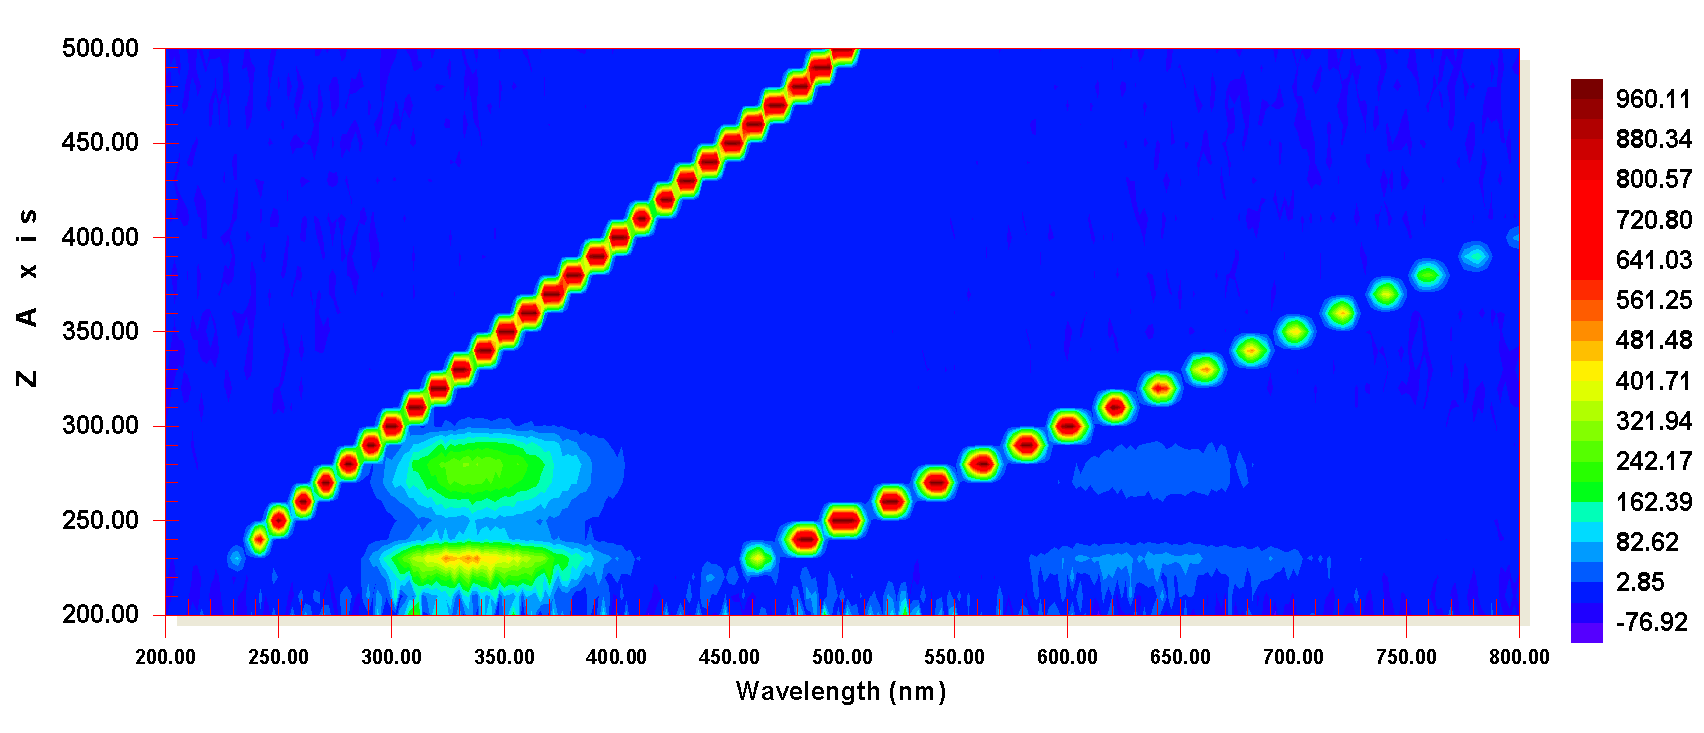
\includegraphics[width=0.98\textwidth]{1_main_matter/co2hb_figures/fluorescence_matrices/coarse/o2.png}
	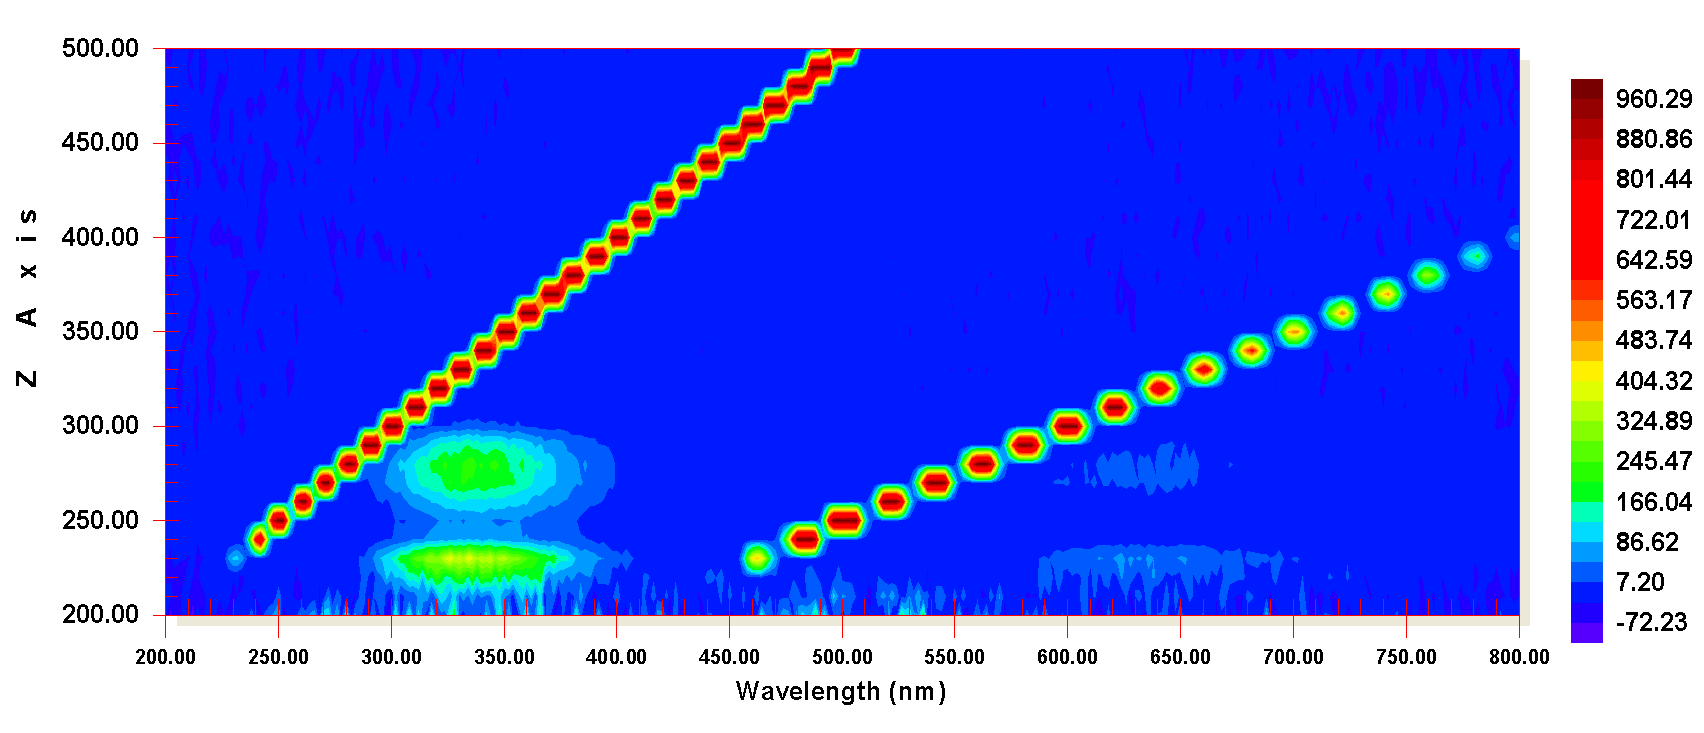
\includegraphics[width=0.98\textwidth]{1_main_matter/co2hb_figures/fluorescence_matrices/coarse/n2.png}
	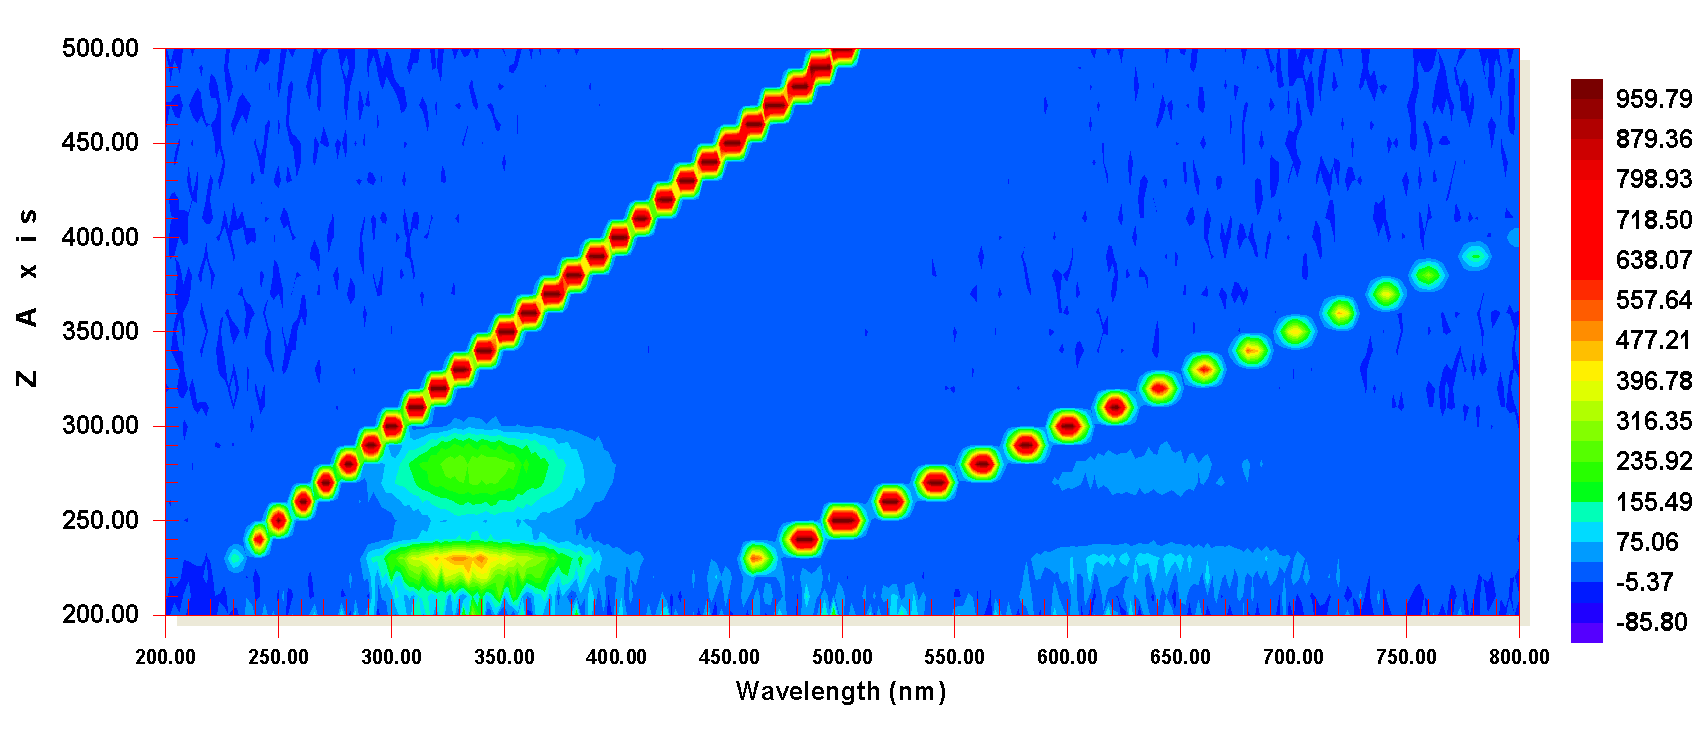
\includegraphics[width=0.98\textwidth]{1_main_matter/co2hb_figures/fluorescence_matrices/coarse/co2.png}
	\caption[Coarse-grained haemoglobin fluorescence matrices.]{Coarse-grained (10~nm excitation step) fluorescence matrices measured on 1:500 diluted lysed blood tonometered with three different gases. The area of interest is that located between the two diagonal lines corresponding to the excitation and its second harmonic. \textbf{Top:} \gls{o2hb} (air). \textbf{Middle:} \gls{hb} (\gls{n2}). \textbf{Bottom:} \gls{co2hb} (\gls{co2}).}
	\label{fig:co2hb:fluo_matrix_coarse}
\end{figure}

\begin{figure}
	\centering
	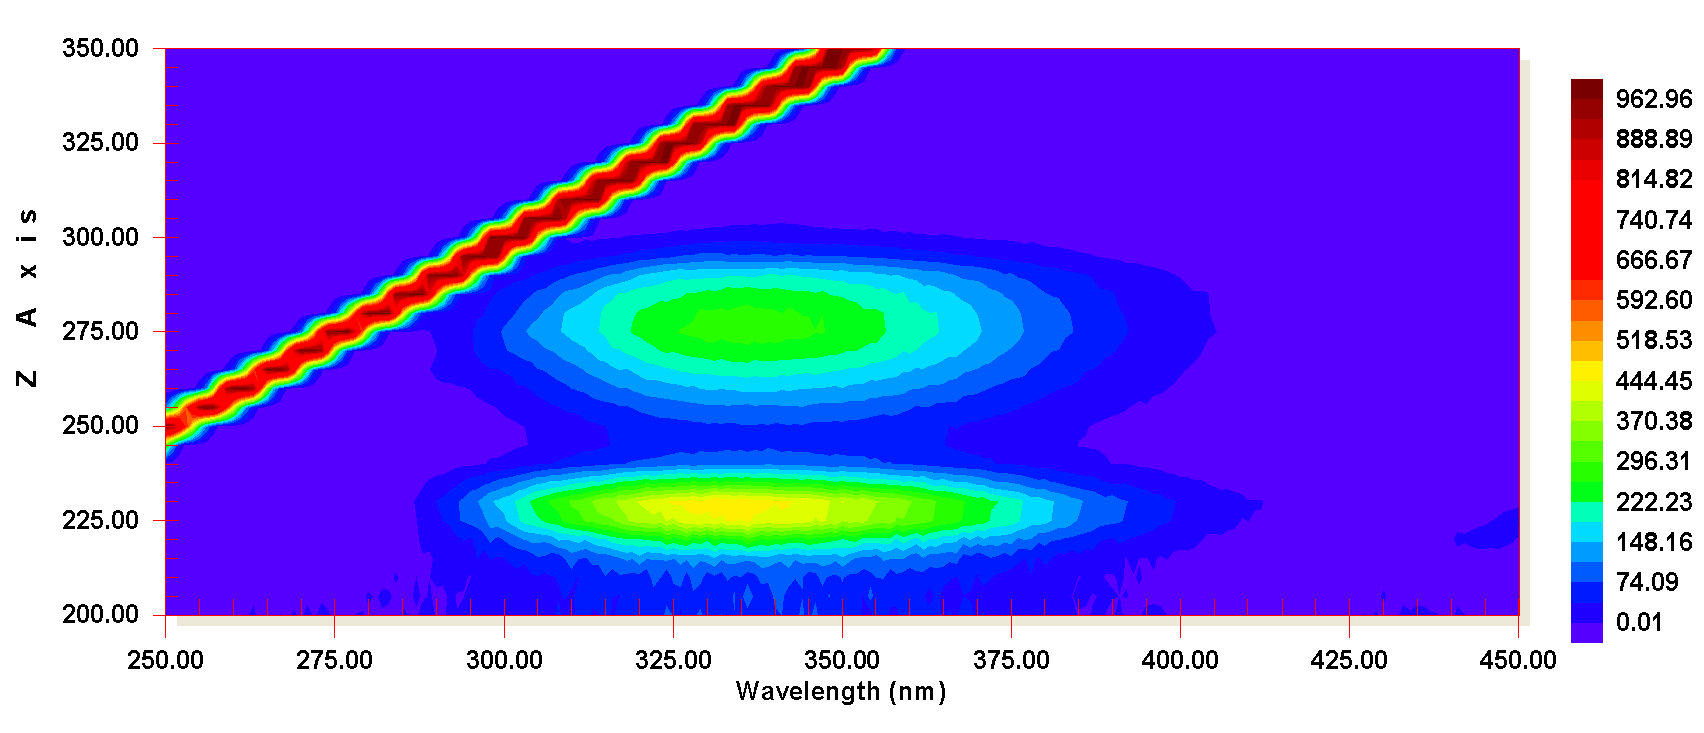
\includegraphics[width=0.98\textwidth]{1_main_matter/co2hb_figures/fluorescence_matrices/fine/o2.png}
	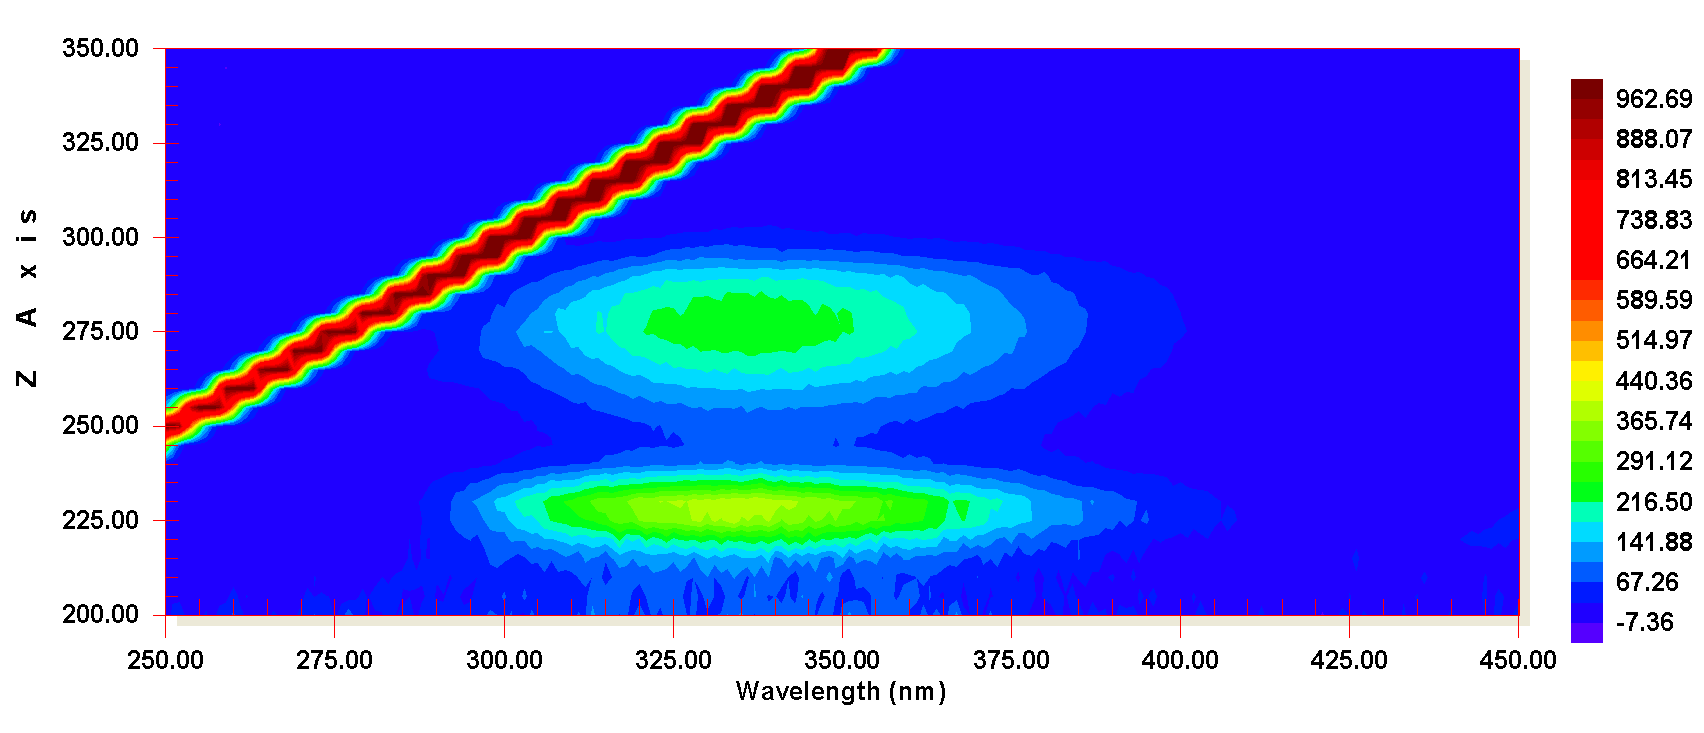
\includegraphics[width=0.98\textwidth]{1_main_matter/co2hb_figures/fluorescence_matrices/fine/n2.png}
	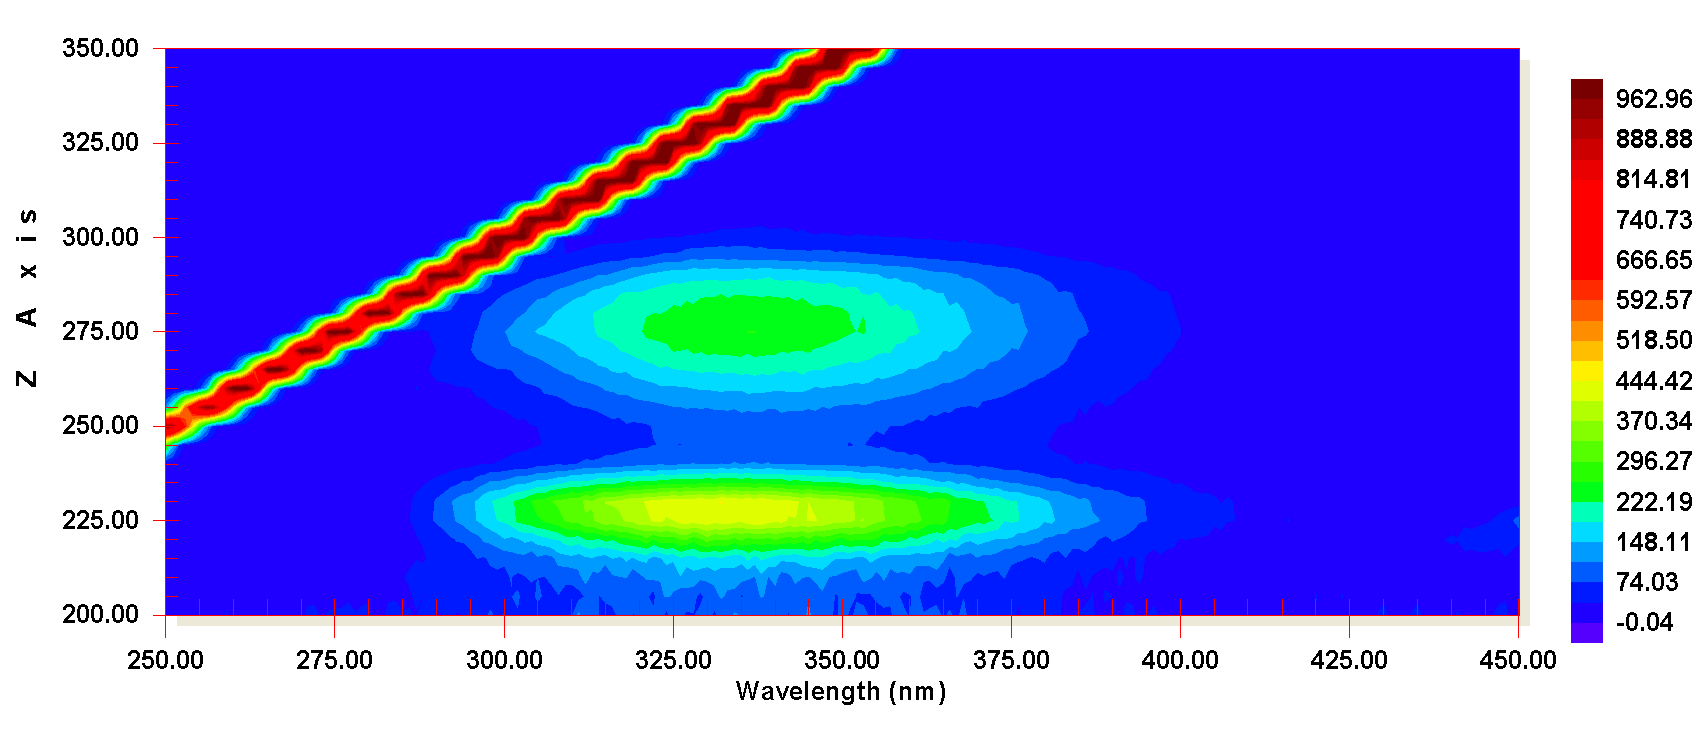
\includegraphics[width=0.98\textwidth]{1_main_matter/co2hb_figures/fluorescence_matrices/fine/co2.png}
	\caption[Fine-grained haemoglobin fluorescence matrices.]{Fine grained (2 nm excitation step) fluorescence matrices measured on 1:500 diluted lysed blood tonometered with three different gases. \textbf{Top:} \gls{o2hb} (air). \textbf{Middle:} \gls{hb} (\gls{n2}). \textbf{Bottom:} \gls{co2hb} (\gls{co2}).}
	\label{fig:co2hb:fluo_matrix_fine}
\end{figure}

\begin{figure}
	\centering
	\includegraphics{1_main_matter/co2hb_figures/tikz/out/o2hb_fluo_spectra.pdf}
	\caption[\gls{o2hb} excitation and emission spectra.]{\gls{o2hb} excitation and emission spectra. The excitation spectrum at $\lambda_\text{em}$ = 336~nm exhibits two maxima at 228 and 278~nm, at which the corresponding emission spectra were measured.}
	\label{fig:co2hb:o2hb_fluo_spectra}
\end{figure}

Two excitation maxima were identified at 228~nm and 278~nm, leading to a single emission peak at 336~nm. Those results are in good agreement with that of the aforementioned literature\cite{hirsch1980, alpert1980}. However, we did not perform enough measurements to be able to conclude on a difference between \gls{o2hb} and \gls{hb} fluorescence spectra, due to a measurement error on our side in the same order of magnitude as the difference reported by Itoh \etal{}\cite{itoh1981} or Hirsch \textit{et al.}\cite{hirsch1981}. By performing such measurement, our aim was mainly to be sure that no other haemoglobin fluorescence existed apart from that already reported elsewhere.

\subsubsection{Other Endogenous Fluorophore}

When performing optical measurements \invivo{}, one should also take into account the presence of other endogenous fluorophores. Several reviews were written on the topic\cite{wagnieres1998, vishwanath2011} and it appears than many fluorescent compounds are naturally present in human tissues. These fluorophores are most likely to interfere with haemoglobin fluorescence measurements, as can be seen in Figure~\ref{fig:co2hb:wagnieres_fig}. Of particular interest, haemoglobin is only considered as an absorber---and not as a potential source of fluorescence---in most fluorescence studies using endogenous fluorophores. One might thus expect its emission to be much lower than that of most other endogenous fluorophores\cite{kollias2002}.

\begin{figure}
	\centering
	\includegraphics{1_main_matter/co2hb_figures/tikz/out/wagnieres.pdf}
	\caption[Fluorescence excitation and emission spectra of various endogenous tissues fluorophores.]{Fluorescence excitation (left) and emission (right) spectra of various endogenous tissues fluorophores. Drawn using data from \cite{wagnieres1998}.}
	\label{fig:co2hb:wagnieres_fig}
\end{figure}

Other studies focused on more specific media such as blood, erythrocyte, or serum. Wolfbeis \etal{}, for instance, measured the fluorescence spectrum of human serum, which exhibits a strong fluorescence corresponding to that of tryptophan, but otherwise weakly fluoresces\cite{wolfbeis1985}. Gao \textit{et al.}\cite{gao2004}, for their part, wrote a brief letter indicating the strong fluorescence of mouse blood---and especially erythrocytes---under a 457.9~nm excitation from Ar$^+$ laser. Alas, the authors did not specify the state of oxygenation of the blood that they used.

On the same topic, Saytashev \textit{et al.}\cite{saytashev2016} used two-photon excitation fluorescence on one hand, and third harmonic generation\footnote{A non-linear optic propagation phenomenon, which generates several harmonics of a fundamental excitation frequency.} on the other hand, to study the fluorescence of erythrocytes through transfusion blood bag membranes made out of \gls{pvc}. They used a Ti-Sapphire 800~nm laser for two-photon excitation fluorescence and a Yb-Fiber 1060~nm laser for third harmonic excitation. They also used a combination of both to equates a 430~nm excitation. The authors performed imaging of the erythrocytes through the plastic bag membrane but could only \enquote{see} through one layer of erythrocytes---due to strong optical absorption of the latter.

Finally, from a more clinical point of view, fluorescence can also be used to probe suspicious tissues for the presence of cancerous cells. As soon as 1987, Yuanlong \etal{}\cite{yuanlong1987} noticed that variations in fluorescence intensity---probably due to local variations in tryptophan content---exist between tumorous and healthy tissues. These differences were confirmed in acetone extracts and relate well to that caused by variations in porphyrin concentration. Masilamani \etal{} also studied the effect of cancer on fluorescence spectra of acetone-extracts of tumorous blood in 2004\cite{masilamani2004}, and their results were later confirmed by Lualdi \etal{} in 2007\cite{lualdi2007}, and by themselves in 2012\cite{masilamani2012}.


\subsubsection{Light Penetration in Tissues}\label{sect:co2hb:light_pene}

Transcutaneous optical measurements have been widely used over the past decades to gain physiological insights into the physiological or clinical state of a subject---\eg{} in the context of pulse oximetry, as exposed in Section~\ref{sect:co2hb:pulse_oximetry}. However, such measurements always take place within the so-called \enquote{optical-window} of the tissues---\ie{} in the 600--1000~nm range---wherein the absorptions of haemoglobin, water, and melanin are low enough to allow for light at these wavelengths to penetrate several millimetres deep inside the tissues. Indeed, from infrared wavelengths up to 630~nm, one can expect a light penetration depth in the 2--6~mm range for an attenuation factor from $1/e$ to $1/100$, depending on the authors\cite{wilson1985, melo2001, ash2017}.

Alas, things turn sour as the excitation wavelength shortens. For instance, when Bruls \textit{et al.}\cite{bruls1984} published their measurements of light transmission in human stratum corneum and epidermis, they reported an exceedingly low transmission of human skin upper layers in the ultraviolet range, with less than 5\% of transmitted light at a 60~\textmu{}m depth, using a 297~nm wavelength. These 5\% can be compared with 53\% of transmitted light at the same depth for a 546~nm incident radiation. Similar studies reported penetration depths\footnote{Defined in this very example as that required to reach a tenfold attenuation. Various authors tend to use the expression \enquote{penetration depth} for quite different attenuation factors---\eg{} $1/e$, $1/3$, $1/10$, $1/100$, \etc{}.} of less than 200~\textmu{}m for excitation wavelengths of 400--450~nm\cite{gmitro1988, koenig1998, barun2007}. These results might be explained by the strong absorbance in the ultraviolet region of the spectrum exhibited by most skin chromophores\cite{young1997}.

Yet, other authors such as Sinichkin \etal{} are less pessimistic: in a study on the fluorescence and attenuation of light in the upper layers of human skin---including the influence of an external pressure on the tissues---the authors concluded that no light penetration can occur deeper than 800~\textmu{}m at 337~nm and 1500~\textmu{}m at 460~nm\cite{sinichkin1998}.

\begin{figure}
	\centering
	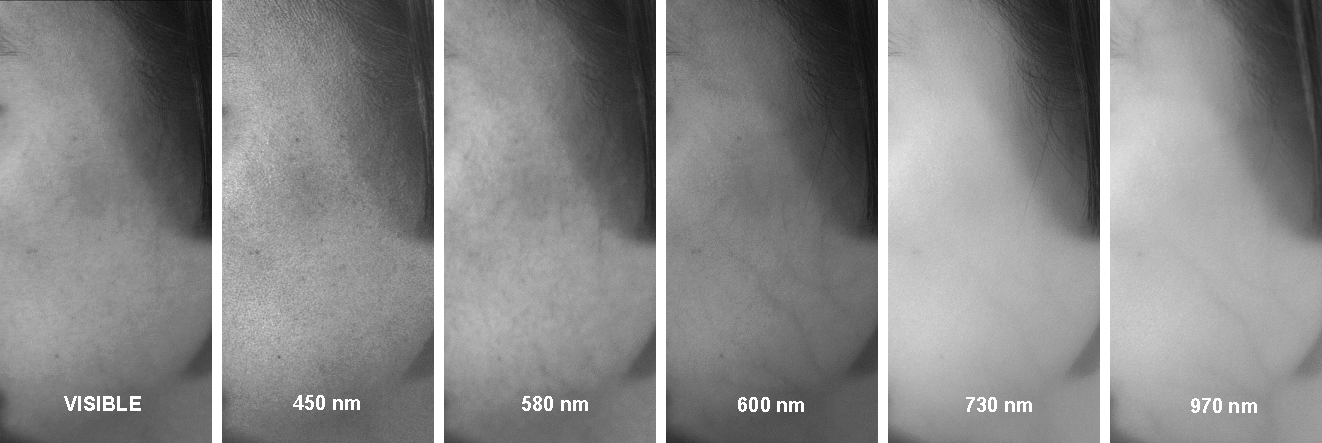
\includegraphics[width=\linewidth]{1_main_matter/co2hb_figures/stamatas_hs.png}
	\caption[Hyperspectral image of a volunteer's face at different wavelengths.]{Hyperspectral image of a volunteer's face at different wavelengths. Private communication from Georgios Stamatas, a modified version of this picture was previously published in \cite{stamatas2003}.}
	\label{fig:co2hb:stamatas_fig}
\end{figure}

Finally, on a more visual scale, Stamatas \etal{}\cite{stamatas2003} performed hyperspectral imaging on a volunteer's cheek. One can see in Figure \ref{fig:co2hb:stamatas_fig} that at 580~nm the veins and capillary underneath the skin are clearly visible, demonstrating that light penetrates the tissues quite deep at this wavelength. However, the latter capillary bed becomes invisible at 450~nm---even if the haemoglobin optical density at this wavelength is extremely high---the upper layers of the skin preventing all the incident light from penetrating into the tissues.

\subsection{Discussion}

We stated earlier in Section~\ref{sect:co2hb:fluo:prev_work} that three main requirements needed to be fulfilled in order to make transcutaneous haemoglobin fluorescence measurements feasible. Those three arguments are reconsidered below in light of the afore-presented bibliography:

\begin{itemize}
	\item[--] \textbf{the haemoglobin fluorescence} is extremely weak, explaining its absence of measurement until the eighties, either when using front-face optics with relatively dilute solutions ($\sim$0.1~mM)\cite{hirsch1980}, or when using extremely dilute solution (2~\textmu{}M) with more conventional right-angled optics\cite{alpert1980}. This fluorescence weakness is justified by the above-mentioned self-quenching phenomenon, which makes fluorescence hardly detectable in concentrated haemoglobin solutions such as blood. In particular, the saturation of haemoglobin fluorescence for concentration above 0.16~mM observed by Hirsch \etal{}\cite{hirsch1980} reveals that---at high concentration---any fluorescence measured from a haemoglobin solution predominantly emanates from the thin layer of the solution present at the surface of its container. For reference, taking a normal haemoglobin concentration in blood of 13--15~g.dL$^{-1}$\cite{us_hematological2005} translates into about 2~mM---more than tenfold the upper limit given by Hirsch.
	\item[--] \textbf{the surrounding medium}---for instance blood serum or other tissues---contains many other fluorophores or chromophores---\eg{} porphyrins, \gls{nadh}, collagen or elastin. In all the available studies which listed such compounds and characterised their fluorescence, haemoglobin was always considered only as a quencher, showing no measurable fluorescence compared to that of other species\cite{wolfbeis1985, wagnieres1998, kollias2002, vishwanath2011}.
	\item[--] \textbf{the probed tissues} and especially the upper layers of the skin, are translucent in the 600--1000~nm optical window. However they become more and more opaque as the wavelength shortens and most authors reported a depth of penetration of at most 60--200~\textmu{}m on the 300--450~nm range\cite{bruls1984, gmitro1988, koenig1998, barun2007, young1997}. Even if Sinichkin \etal{} argue of higher values up to 1500~\textmu{}m\cite{sinichkin1998}, such values are still way below that reported at the lower wavelengths usually selected for pulse oximetry.
\end{itemize}

\paragraph{Conclusion:} facing such facts, we concluded that haemoglobin transcutaneous fluorescence measurements are but a lost cause. Thus, we did not push our experimentations any further to determine whether the fluorescence spectra of \gls{hb}, \gls{o2hb}, or \gls{co2hb} do actually differ or not.

\section{Conclusion}\label{sect:co2hb:conclusion}

In humans, blood gases are transported through several pathways: \gls{o2} is carried both as a dissolved gas and bound to haemoglobin, while \gls{co2} is transported in these same forms as well as in the form of bicarbonate ions and carbamates---Section~\ref{sect:co2hb:blood_gases}. One interesting feature of haemoglobin is its strong optical absorption---the latter gives \myblood{} its vivid red colour---which depends on the oxidation state of the molecule---Section~\ref{sect:co2hb:hb_optical_prop}. This latter difference in the absorption spectra of \gls{hb} and \gls{o2hb} gave rise to blood oximetry in the forties, followed by pulse oximetry in the seventies---Section~\ref{sect:co2hb:pulse_oximetry}. Owing to the global success of the latter technique, and to the recent possibility of embedding it into ubiquitous wearables, I thought that having an equivalent for \gls{co2hb} would be a convenient means to address my doctoral thesis' problematic. However, putting this naive idea into practice would require the absorption spectrum of \gls{co2hb} to be significantly different from that of other haemoglobin species. The above-presented experimentations demonstrated that this is unfortunately not the case, sealing the coffin of pulse carbametry---Section~\ref{sect:co2hb:pulse_carbametry}. Out of curiosity, additional research was performed on haemoglobin fluorescence, but the latter proved to be unusable for \invivo{} transcutaneous measurements---Section~\ref{sect:co2hb:fluo}.

Retrospectively, with hindsight, the chances that \gls{co2hb} and \gls{hb} absorption spectra differed significantly were rather tenuous from the outset. Indeed, changes in the absorption spectra of haemoglobin with its ligation state are the result of conformational changes in the haemoglobin molecule itself\cite{antonini1970}. Details on these changes have been well-documented by a number of authors\cite{perutz1964, paoli1996, park2006hb, bringas2017} and Yuan \etal{} recently wrote a thorough review on this very topic\cite{yuan2015}. However, no change of the same order of magnitude seems to happen when \gls{co2} binds to haemoglobin's amino groups. To the best of my knowledge, only Arnone \etal{} studied the tenuous structural changes of \gls{hb} upon \gls{co2} binding, concluding that \enquote{\gls{co2} binding does not result in major changes in $\beta$ chain tertiary structure}\cite{arnone1980}---knowing that $\alpha$ chains \gls{co2}-binding is even weaker than that of $\beta$ chains. This lack of major structural change of haemoglobin upon \gls{co2} binding in turns likely explains why \gls{hb} and \gls{co2hb} absorption spectra are so close to each other\footnote{As the compassionate reader can imagine, I was not aware of the state of affair described in this latter paragraph until years after having performed my original \gls{co2hb} spectrum measurements.}.

Following this conclusion, I decided to reorient my research towards transcutaneous \gls{co2} diffusion, as discussed in the following chapters. Of note, I recently conducted \gls{nir} measurements of \gls{o2hb}, \gls{hb}, \gls{cohb}, \gls{co2hb} and \gls{methb} spectra on the 600--2350~nm range. Due to the shortness of time and the non-trivial extraction of haemoglobin absorption spectra from raw measurements---mainly caused by the significant absorption of water above 1300~nm---these measurements are not included in this doctoral work. From a very qualitative point of view, these measurement yielded \gls{hb} and \gls{co2hb} absorption spectra that were identical to the naked eye---as strongly expected. A more rigorous and quantitative analysis should be published soon---\ie{} by early 2025 approximately---so \href{https://wayback-api.archive.org/web/20240612134342/https://scholar.google.fr/citations?user=DCR_h9YAAAAJ&hl=fr}{stay} \href{https://wayback-api.archive.org/web/20240612134527/https://www.researchgate.net/profile/Emmanuel-Dervieux-2}{tuned}.